\documentclass[authoryear]{elsarticle}

\usepackage[utf8]{inputenc}
%\usepackage[english,russian]{babel}

\usepackage{amsmath}
\usepackage{bm}
\usepackage{tikz}
\usepackage{pgfplots}
\usepackage{color, colortbl}
\usepackage{graphicx}

\definecolor{col1}{gray}{0.8}
\definecolor{col2}{gray}{0.9}
\definecolor{col3}{gray}{0.95}

\usepackage{hyperref}

\newtheorem{thm}{Theorem}
\newtheorem{lem}[thm]{Lemma}
\newproof{pf}{Proof}

\journal{Annals of Nuclear Energy}

\bibliographystyle{elsarticle-harv}

\begin{document}

\begin{frontmatter}

%\title{Спектральные характеристики динамических процессов в ядерном реакторе}

\author[ki]{Alexander V. Avvakumov}
\ead{Avvakumov2009@rambler.ru}

\author[nsi]{Valery~F.~Strizhov\corref{cor}}
\ead{vfs@ibrae.ac.ru}

\author[nsi,univ]{Petr N. Vabishchevich}
\ead{vabishchevich@gmail.com}

\author[univ]{Alexander O. Vasilev}
\ead{haska87@gmail.com}

\address[ki]{National Research Center \emph{Kurchatov Institute},  1, Sq. Academician Kurchatov, Moscow, Russia}
\address[nsi]{Nuclear Safety Institute, Russian Academy of Sciences, 52, B. Tulskaya, Moscow, Russia}
\address[univ]{North-Eastern Federal University, 58, Belinskogo, Yakutsk, Russia}

\cortext[cor]{Corresponding author}

\begin{abstract}
%Моделирование динамических процессов в ядерных реакторах проводиться, чаще всего,
%на основе описания нейтронного потока в многогрупповом диффузионном приближении.
%Базовая модель включает многомерную систему связанных уравнений параболического типа.
%По аналогии с обычными тепловыми процессами можно выделить регулярный режим
%работы ядерного реактора, который связан с самоподобным развитием нейтронного поля
%при больших временах. Основной характеристикой динамических процессов
%выступает минимальное собственное значение соответствующей спектральной задачи.
%Приведены результаты расчета различных собственных значений в рамках двухгруппового приближения 
%численного теста для реактора на тепловых нейтронах ВВЭР-1000.
\end{abstract}

\begin{keyword}

Neutron diffusion equation \sep  multi-group approximation \sep space-time kinetic 
\sep spectral problem \sep regular regime of time-dependent process.

\end{keyword}

\end{frontmatter}


\section{Introduction} 
The physical processes in a nuclear reactor \cite{duderstadt1976nuclear}
depend on distribution of neutron flux, whose mathematical description is based on the neutron-transport equation
\cite{hetrick1971dynamics,stacey}. 
The general view of this equation is integrally-differential one, and the required distribution of neutrons flux depends on time, energy, spatial and angular variables. As a rule, the simplified forms of the neutron transport equation are used for practical calculations of nuclear reactors. The equation system that is known as a multigroup diffusion approach is mostly used for reactor analysis
\cite{marchuk1986numerical,lewis1993computational,sutton1996diffusion,cho2005fundamentals}
and is applied in most engineering calculation codes.

The standard methods of approximate solutions of non-stationary problems are used for modelling of the dynamics of neutron-physical processes. The most attention is paid to two-layer schemes with weights ($\theta$-method)
\cite{Ascher2008,LeVeque2007,HundsdorferVerwer2003},
the Runge-Kutta and Rosenbrock schemes 
\cite{Butcher2008,HairerWanner2010} are used.
Let’s note a special class of methods for modelling of non-stationary neutron transport in diffusion multigroup approximation, which is connected with multiplicate representation of solution --- space-time factorization methods and the quasistatic method
\cite{chou1990three,dahmani20013d,dodds1976accuracy,goluoglu2001time}.
The approximate solution is searched in the form of two functions product, one of which depends on time and is related to the amplitude, the second one (the shape function) describes the spatial distribution. It is difficult to check the accuracy of the approximate solution in such approach, in particular, while calculating the dynamic modes with the complex transformation of the density field of neutron flux.

The processes in a nuclear reactor are essentially non-stationary. The stationary state of neutron flux, which is related to the critical state of the reactor, is characterised by local balancing of neutron absorption and birth intensities. This boundary state is usually described by solution of a spectral problem (Lambda Modes problem, $\lambda$-eigenvalue problem) provided that the fundamental eigenvalue (maximal eigenvalue) that is called k-effective of the reactor core, is equal to unity. In this case, the stationary neutron field is a corresponding eigenfunction. Calculations of k-effective of the reactor on the basis of the spectral Lambda Modes problem solution are obligatory for developing a new design of reactor installation.

Time behaviour of nuclear reactor is deemed sometimes to be related to the deviation of k-effective from unity that involves, in particular, concept of reactivity. This is not justified, since, while calculating this parameter, the evolutionary nature of neutron redistribution processes (nonstationary systems of the equations) is considered in no way. The k-effective parameter deviates from unity, though quite weakly, but anyway such a solution, generally speaking, cannot be connected with the stationary solution of the problem. There is simply no such a solution. Thus, the attempts to correct the basic mathematical model of non-stationary neutron diffusion by introducing some correcting multipliers to achieve the strict criticality are not successful.

The spectral parameter $\alpha$, which is not directly connected with k-effective, is proposed to be used instead of k-effective for more adequate characteristic of the dynamic nature of reactor. It is defined as the fundamental eigenvalue of the spectral problem (time-eigenvalue, $\alpha$-eigenvalue problem), which is connected with the non-stationary equations of neutron diffusion
\cite{Bell1970,modak2007scheme,verdu20103d}.
By analogy with the usual problems of heat conductivity (see, for example,
\cite{luikov2012analytical,samarskii1996computational}) we consider the regular reactor mode. At the large values of time, the behaviour of a neutron field is asymptotic, and one can talk about space-time factorization solution, whose amplitude is $\exp(\alpha t)$, the shape function is the eigenfunction of the spectral problem. 

Study of the dynamic processes can be based on the discrimination of symmetric and skew-symmetrical parts of the neutron transport operator. In this case, we can easily get the aprioristic assessments of stability in the corresponding norm, while assessing the operator of the symmetric part from below, and perform the analysis of used time approximations
\cite{Samarskiibook,SamarskiiMatusVabischevich2002}. 
To get this, the partial spectral problem is solved to find the fundamental eigenvalue $\delta$ of the Delta Modes spectral problem.

The paper is organised as follows. The statement of the boundary-value problem for the system of non-stationary diffusion equations in multigroup approach is given in Section 2. Various spectral problems are discussed in Section 3. A numerical example of calculation of spectral characteristics within the frameworks of two-dimensional tests problem for VVER-1000 reactor and HWR reactor using the two-group system of diffusion equations is discussed in Section 4. The results of the work are summarised in Section 5.

\section{Problem statement}

The neutron field is modelled in multigroup diffusion approximation. The neutron dynamics is considered in the limited convex two-dimensional or three-dimensional area  $\Omega$ ($\bm x = \{x_1, ..., x_d\} \in \Omega, \ d = 2,3$) with boundary $\partial \Omega$. The neutron transport is described by the system of equations:
\begin{equation}\label{1}
\begin{split}
 \frac{1}{v_g} \frac{\partial \phi_g}{\partial t} - & \nabla \cdot D_g \nabla \phi_g + \Sigma_{rg} \phi_g 
 - \sum_{g\neq g'=1}^{G} \Sigma_{s,g'\rightarrow g} \phi_{g'} \\
 =  & \ (1-\beta) \chi_g \sum_{g'=1}^{G} \nu \Sigma_{fg'} \phi_{g'} + \widetilde{\chi}_g \sum_{m=1}^{M} \lambda_m c_m , \quad 
 g = 1,2, ..., G .
\end{split}
\end{equation} 
Here $\phi_g(\bm x,t)$ --- neutron flux of $g$ group at point $\bm x$ and time $t$,
$G$ --- number of groups,
$v_g$ --- effective velocity of neutrons in the group $g$,
$D_g(\bm x)$ --- diffusion coefficient, $\Sigma_{rg}(\bm x,t)$ --- removal cross-section,
$\Sigma_{s,g'\rightarrow g}(\bm x,t)$ --- scattering cross-section from group $g'$ to group $g$,
$\beta$ --- effective fraction of delayed neutrons, $\chi_g$, $\widetilde{\chi}_g$  --- spectra of instantaneous and delayed neutrons, 
$\nu\Sigma_{fg}(\bm x,t)$ --- generation cross-section of group $g$,
$c_m$ --- density of sources of delayed  $m$-type neutrons,  $\lambda_m$ --- decay constant of sources of delayed neutrons,
$M$ --- number of types of delayed neutrons.
The density of sources of delayed neutrons is described by the equations:
\begin{equation}\label{2}
 \frac{\partial c_m}{\partial t} + \lambda_m c_m = \beta_m \sum_{g=1}^{G} \nu \Sigma_{fg} \phi_g ,
 \quad m = 1,2, ..., M , 
\end{equation} 
where $\beta_m$ --- is a fraction of delayed $m$-type neutrons, and
\[
 \beta = \sum_{m=1}^{M} \beta_m .
\] 
System of equations (\ref{1}), (\ref{2}) is supplemented with corresponding initial and boundary conditions.

The albedo-type conditions are set at the boundary of the area $\partial \Omega$:
\begin{equation}\label{3}
 D_g\frac{\partial \phi_g}{\partial n} + \gamma_g \phi_g = 0, \quad 
 \quad g = 1,2, ..., G ,
\end{equation}
where $n$ --- outer normal to the boundary $\partial \Omega$.

Let’s propose that in the initial time moment (at $t=0$) the reactor is in the critical state:
\begin{equation}\label{4}
 \phi_g(\bm x,0) = \phi_g^0(\bm x), 
 \quad c_m(\bm x,0) = c_m^0(\bm x) . 
\end{equation} 
For $\phi_g^0(\bm x)$ and $c_m^0(\bm x)$ we get:
\[
 \begin{split}
 - \nabla \cdot D_g \nabla \phi_g^0 & + \Sigma_{rg} \phi_g^0 
 - \sum_{g\neq g'=1}^{g-1} \Sigma_{s,g'\rightarrow g} \phi_{g'}^0 \\
 & = ( (1-\beta) \chi_g + \beta \widetilde{\chi}_g) \sum_{g'=1}^{G} \nu \Sigma_{fg'} \phi_{g'}^0 , \quad 
 g = 1,2, ..., G ,
\end{split}
\] 
\[
 \lambda_m c_m^0 = \beta_m \sum_{g=1}^{G} \nu \Sigma_{fg} \phi_g^0 ,
 \quad m = 1,2, ..., M .
\] 

It is possible to limit the problem for neutron flux without considering the delayed neutrons, when instead of  (\ref{1}) we obtain the following equation:
 \begin{equation}\label{5}
\begin{split}
 \frac{1}{v_g} \frac{\partial \phi_g}{\partial t} - & \nabla \cdot D_g \nabla \phi_g + \Sigma_{rg} \phi_g 
 - \sum_{g\neq g'=1}^{G} \Sigma_{s,g'\rightarrow g} \phi_{g'} \\
 =  & \ ( (1-\beta) \chi_g + \beta \widetilde{\chi}_g) \sum_{g'=1}^{G} \nu \Sigma_{fg'} \phi_{g'} , \quad 
 g = 1,2, ..., G .
\end{split}
\end{equation} 
The problem for equation (\ref{5}) is solved with boundary conditions of form (\ref{3})and the following initial conditions:
\begin{equation}\label{6}
 \phi_g(\bm x,0) = \phi_g^0(\bm x), 
 \quad  g = 1,2, ..., G .
\end{equation} 

Let’s write the boundary problem (\ref{3}), (\ref{5}), (\ref{6}) in operator form. The vector $\bm \phi = \{\phi_1, \phi_2, ..., \phi_G\}$ and matrices are defined as follows:
\[
 V = (v_{g g'}),
 \quad v_{g g'} = \delta_{g g'} v_g^{-1},
\] 
\[
 D = (d_{g g'}),
 \quad d_{g g'} = - \delta_{g g'} \nabla \cdot D_g \nabla,
\] 
\[
 S = (s_{g g'}),
 \quad  s_{g g'} =  \delta_{g g'} \Sigma_{rg} - \Sigma_{s,g'\rightarrow g} ,
\] 
\[
 R = (r_{g g'}),
 \quad  r_{g g'} = ( (1-\beta) \chi_g + \beta \widetilde{\chi}_g) \nu \Sigma_{fg'} ,
\]
\[
g, g' = 1,2, ..., G,
\] 
where
\[
 \delta_{g g'} = \left \{ 
 \begin{matrix}
 1, & g = g', \\
 0, & g \neq  g',
 \end{matrix}
 \right . 
\] 
is the Kronecker delta.
We shall use the set of vectors $\bm \phi$, whose components satisfy the boundary conditions (\ref{3}). Using the set definitions, the system of equations (\ref{5}) ) can be written in the form of first-order equation of evolution:
\begin{equation}\label{7}
 V \frac{d \bm \phi}{d t} + (D+S) \bm \phi = R \bm \phi .
\end{equation}  
The Cauchy problem is solved for (\ref{7}), when
\begin{equation}\label{8}
 \bm \phi(0) = \bm \phi^0,
\end{equation} 
where (see (\ref{6})) $\bm \phi^0 = \{ \phi_1^0,  \phi_2^0, ...,  \phi_G^0 \}$.

\section{Spectral problems} 

To characterize the dynamic processes in a nuclear reactor, which are described by Cauchy problem (\ref{7}), (\ref{8}), solutions of some spectral problems  \cite{Bell1970,hetrick1971dynamics,stacey}.

The following spectral problem is usually solved:
\begin{equation}\label{9}
 (D+S) \bm \varphi  = \lambda^{(k)} R \bm \varphi .
\end{equation} 
This problem (\ref{9}) is known as the Lambda modes problem for a given configuration of the reactor core.
The minimal eigenvalue is used for characterisation of neutron field, thus 
\[
 k = \frac{1}{\lambda^{(k)}_1}  
\] 
is the effective multiplication factor.
The value $k = \lambda^{(k)}_1 = 1$ is related to the critical state of the reactor, and the corresponding eigenfunction $\varphi_1(\bm x)$ is the stationary solution of the equation (\ref{7}).
At $k > 1$, one can speak about supercriticality, at $k < 1$  --- about subcriticality.

Due to nonself-adjoint operators of neutron transport we have, generally speaking, the complex eigenvalues. The reality and positivity property of the fundamental eigenvalue for the system of neutronics equations is proved using the principle of maximum at some restrictions on factors of neutron transport operators  \cite{habetler1961existence}. 
This is also true for the nonself-adjoint elliptic operator of the second order \cite{bookEvans}. 

The spectral problem (\ref{9}) cannot directly be connected with the dynamic processes in a nuclear reactor. At the best, we can get only the utmost case --- the stationary critical state.The more acceptable spectral characteristics for the non-stationary equation (\ref{7}) are related the the spectral problem 
\begin{equation}\label{10}
 A \bm \varphi  =  \lambda^{(\alpha)} V \bm \varphi ,
 \quad A = D + S - R . 
\end{equation} 
The fundamental eigenvalue 
\[ 
 \alpha = \lambda^{(\alpha)}_1
\]
is called \cite{Bell1970}
$\alpha$--eigenvalues and as period eigenvalues,
because they are inversely related to the reactor periods.
The asymptotic behaviour of Cauchy problem solution (\ref{7}), (\ref{8}) at large times can be connected connect with the eigenvalue $\alpha$.
In this regular mode, the reactor behaviour is described by the function $\exp(-\alpha t) \varphi_1(\bm x)$.
Critical state of the reactor is defined by the values $\alpha = 0$; when $\alpha > 0$ we get the supercritical state, and when $\alpha <  0$ --- – subcritical state of the reactor.

A priori assessments of solution at the current time are used to characterize the evolution processes \cite{bookEvans}. Let’s define the Hilbert space $H = \bm L_2(\Omega)$, for vector functions, in which the scalar product $(\cdot, \cdot)$  and norm $\|\cdot \|$ are as follows:
\[
 (\bm \phi , \bm \varphi) = \sum_{g=1}^{G} (\phi_g, \varphi_g) ,
 \quad \|\bm \phi \| = (\bm \phi , \bm \phi)^{1/2} ,
\] 
where
\[
 (\phi_g, \varphi_g) = \int_{\Omega} \phi_g (\bm x) \varphi_g (\bm x) \, d \bm x ,
 \quad g = 1,2, ..., G . 
\] 
Let’s select the self-adjoint and skew-symmetric parts in the operator $A$:
\[
 A = A_1 + A_2, 
 \quad A_1 = A_1^* = \frac{1}{2} (A + A^*), 
 \quad A_2 = - A_2^* = \frac{1}{2} (A - A^*) .
\]
The diffusion operator $D$ is self-adjoint at the set of functions satisfying the boundary conditions (\ref{3}): $D = D^*$. For $A_1$ and $A_2$ we get
\[
 A_1 = (a^{(1)}_{g g'}), 
 \quad A_2 = (a^{(2)}_{g g'}),
\]
\[
\begin{split}
 a^{(1)}_{g g'} = & - \delta_{g g'} \nabla \cdot D_g \nabla
 +  \delta_{g g'} \Sigma_{rg} 
 -  \frac{1}{2} \left ( \Sigma_{s,g'\rightarrow g} + \Sigma_{s,g\rightarrow g'} \right ) \\
 & - \frac{1}{2} \left ( ( (1-\beta) \chi_g + \beta \widetilde{\chi}_g) \nu \Sigma_{fg'} 
 + ( (1-\beta) \chi_{g'} + \beta \widetilde{\chi}_{g'}) \nu \Sigma_{fg} \right ) ,
\end{split}
\] 
\[
\begin{split}
  a^{(2)}_{g g'} = & - 
 \frac{1}{2} \left ( \Sigma_{s,g'\rightarrow g} - \Sigma_{s,g\rightarrow g'} \right ) \\
 & - \frac{1}{2} \left ( ( (1-\beta) \chi_g + \beta \widetilde{\chi}_g) \nu \Sigma_{fg'} 
 - ( (1-\beta) \chi_{g'} + \beta \widetilde{\chi}_{g'}) \nu \Sigma_{fg} \right ) .
\end{split}
\] 
Let’s consider the spectral problem
\begin{equation}\label{11}
 A_1 \bm \varphi  =  \lambda^{(\delta)} V \bm \varphi 
\end{equation} 
for the self-adjoint part of the operator $A$. All eigenvalues of the Delta Modes spectral problem (\ref{11}) are real.

Let’s find the fundamental eigenvalue in (\ref{7}), (\ref{8}), to characterize the dynamic processes described by the problem (\ref{11}):
\[
  \delta  = \lambda^{(\delta )}_1,
\] 
and (see, e.g., \cite{Hogben}, section 16.1) $\delta  \leq \alpha$.
Taking into account the skew-symmetry of $A_2$  we obtain
\[
 (A \bm \phi, \bm \phi) = (A_1 \bm \phi, \bm \phi) \geq \delta  (V \bm \phi,\bm \phi),
\] 
i.e.
\begin{equation}\label{12}
 A \geq \delta V . 
\end{equation} 
Based upon the assessment (\ref{12}) the corresponding priori assessment for the Cauchy problem solution (\ref{7}), (\ref{8}) is set. 

Let’s connect the operator $V = V^* > 0$ with the Hilbert space $H_V$, in which the scalar product and norm are
\[
 (\bm \phi , \bm \varphi)_V =  (V \bm \phi , \bm \varphi),
 \quad  \|\bm \phi\|_V =  (V \bm \phi , \bm \phi)_V^{1/2} . 
\] 
Scalar multiplying in $H$ the equation (\ref{7}) by $\bm \phi$ and taking into account (\ref{12}), we obtain:
\[
 \left ( V \frac{d \bm \phi}{d t} , \bm \phi \right ) + \delta (V \bm \phi, \bm \phi ) \leq 0.
\] 
Taking into account
\[
 \left ( V \frac{d \bm \phi}{d t} , \bm \phi \right ) =
 \frac{1}{2} \frac{d}{d t} (V \bm \phi, \bm \phi) = 
 \|\bm \phi\|_V \frac{d }{d t}\|\bm \phi\|_V ,
\] 
we get
\[
 \frac{d }{d t} \|\bm \phi\|_V + \delta \|\bm \phi\|_V \leq 0 .
\] 
Considering the initial condition (\ref{8}), based upon the Grönwall's lemma we come to an aprioristic assessment:
\begin{equation}\label{13}
 \|\bm \phi(t)\|_V \leq \exp (-\delta t ) \|\bm \phi^0\|_V 
\end{equation} 
for the solution of the problem (\ref{7}), (\ref{8}). Such assessments expressing the stability of the solution against the initial data, are the reference points, while constructing the time approximations
\cite{Samarskiibook,SamarskiiMatusVabischevich2002}. 

The spectral problem (\ref{11}) is more convenient for numerical solving than the spectral problems (\ref{9}) and (\ref{10})
\cite{Golubbook,Saadbook}. This is explained by the fact that in this case, all eigenvalues and eigenfunctions are real. The value $\delta$ defines not only the criticality of the reactor (at $\delta = 0$), but also the dynamics of the neutron field of the reactor –-- see the assessment (\ref{13}).

The corresponding spectral problems for the system of equations (\ref{1}), (\ref{2}) are similarly formulated taking into account the delayed neutrons --- total modes \cite{verdu20103d}.
Let’s introduce the vector of density of delayed neutron sources $\bm c = \{c_1, c_2, ..., c_M\}$. The equation (\ref{1}) will be written in the form:
\begin{equation}\label{14}
 V \frac{d \bm \phi}{d t} + (D+S) \bm \phi = R \bm \phi +
 B \bm c,
\end{equation} 
where now
\[
 R = (r_{g g'}),
 \quad  r_{g g'} = (1-\beta) \chi_g ,
 \quad g, g' = 1,2, ..., G,
\] 
and $B$ --- a rectangular matrix:
\[
 B = (b_{gm}),
 \quad  b_{gm} = \widetilde{\chi}_g \lambda_m,
 \quad g = 1,2, ..., G,
 \quad m = 1,2, ....,M .  
\] 
The equation (\ref{2}) in the vector-matrix designations has the form:
\begin{equation}\label{15}
 \frac{d \bm c}{d t} + \Lambda \bm c = Q \bm \phi ,
\end{equation} 
at
\[
 \Lambda = (\lambda_{m m'}),
 \quad  \lambda_{m m'} = \lambda_m \delta_{m m'} ,
 \quad m, m' = 1,2, ....,M ,  
\] 
\[
 Q = (q_{mg}),
 \quad  q_{mg} = \beta_m \nu \Sigma_{fg},
 \quad m = 1,2, ....,M ,  
 \quad g = 1,2, ..., G .
\] 
Initial conditions (\ref{4}) will give
\begin{equation}\label{16}
 \bm \phi(0) = \bm \phi^0,
 \quad  \bm c(0) = \bm c^0,
\end{equation} 
where $\bm c^0 = \{ c_1^0,  c_2^0, ...,  c_M^0 \}$.

The spectral problems that are similar to (\ref{9})--(\ref{11}) are used for characterization of dynamic processes, which are described by the Cauchy problem (\ref{14})--(\ref{16}). The spectral problem (\ref{9}) can be matched with the spectral problem
\[
\begin{split}
 (D+S) \bm \varphi  & = \lambda^{(k)} \left ( R \bm \varphi  +  B \bm s \right ) , \\
 \Lambda \bm s & =  \lambda^{(k)} Q \bm \varphi .
\end{split}
\] 
The spectral problems, for example, of form (\ref{10}) can be formulated similarly. In this case one can get 
\[
\begin{split}
 (D+S - R) \bm \varphi  -  B \bm s & = \lambda^{(\alpha)} V \bm \varphi , \\
 \Lambda \bm s - Q \bm \varphi & =  \lambda^{(\alpha)}   \bm s .
\end{split}
\]
The analogous of the spectral problem (\ref{11}) looks a little be more cumbersome, when the self-adjoint part of the problems operator is separated. 

\section{Numerical examples} 

We shall give some results of eiegnvalue calculation. The elementary two-group model ($G = 2$) is used. With reference to the problem  (\ref{9}) 
one can obtain
\begin{equation}\label{17}
\begin{split}
 - \nabla \cdot D_1 \nabla \varphi_1 & + \Sigma_{r1} \varphi_1  
 = \lambda^{(k)} (\nu \Sigma_{f1} \varphi_1 + \nu \Sigma_{f2} \varphi_2), \\
 - \nabla \cdot D_2 \nabla \varphi_2 & + \Sigma_{r2} \varphi_2 - \Sigma_{s,1\rightarrow 2} \varphi_1  
 = 0.
\end{split}
\end{equation}
Now we give the spectral problem (\ref{10}). Within the used two-group approximation:
\begin{equation}\label{18}
\begin{split}
 - \nabla \cdot D_1 \nabla \varphi_1 & + \Sigma_{r1} \varphi_1    
 - (\nu \Sigma_{f1} \varphi_1 + \nu \Sigma_{f2} \varphi_2) = \lambda^{(\alpha)} \frac{1}{v_1}   \varphi_1, \\
 - \nabla \cdot D_2 \nabla \varphi_2 & + \Sigma_{r2} \varphi_2 - \Sigma_{s,1\rightarrow 2} \varphi_1  
 = \lambda^{(\alpha)} \frac{1}{v_2}   \varphi_2.
\end{split}
\end{equation}
The following problem is compared with the spectral problem (\ref{11}) in two-group approximation:
\begin{equation}\label{19}
\begin{split}
 - \nabla \cdot D_1 \nabla \varphi_1 & + (\Sigma_{r1} - \nu \Sigma_{f1}) \varphi_1 - \frac{1}{2}  (\nu \Sigma_{f2} + \Sigma_{s,1\rightarrow 2}) \varphi_2  = \lambda^{(\delta)} \frac{1}{v_1}   \varphi_1, \\
 - \nabla \cdot D_2 \nabla \varphi_2 & + \Sigma_{r2} \varphi_2 
 - \frac{1}{2}  (\nu \Sigma_{f2} + \Sigma_{s,1\rightarrow 2}) \varphi_1 
 = \lambda^{(\delta )} \frac{1}{v_2}   \varphi_2.
\end{split}
\end{equation} 
The method of finite elements \cite{brenner,quarteroni} 
] on triangular calculation grids is used for the approximate solution of the spectral problem. The number of triangles per one assembly $\kappa$  varies from 6 to 96 (fig.\ref{fig:1}).
The standard Lagrangian finite elements of degree $p=1,2,3$ are used.
The software has been developed using the engineering and scientific calculation library FEniCS \cite{fenics}. SLEPc \cite{hernandez2003resolution,hernandez2005slepc} has been used for numerical solution of the spectral problems.  

\begin{figure}[h]
  \begin{center}
\begin{minipage}{0.30\linewidth}
\center{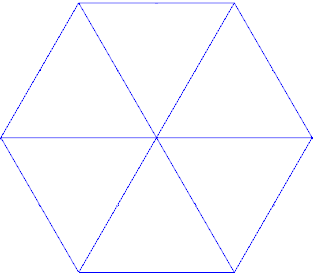
\includegraphics[width=1\linewidth]{1-1.png}}\\
\end{minipage}
\hfill
\begin{minipage}{0.30\linewidth}
\center{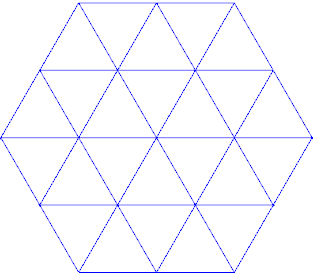
\includegraphics[width=1\linewidth]{1-2.png}}\\
\end{minipage}
\hfill
\begin{minipage}{0.30\linewidth}
\center{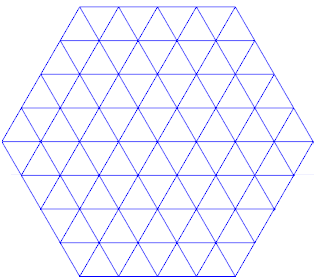
\includegraphics[width=1\linewidth]{1-3.png}}\\
\end{minipage}
\caption{Discretization of assembly into 6, 24 and 96 finite elements.}
\label{fig:1}
  \end{center}
\end{figure}

\subsection{VVER-1000 problem} 
\begin{figure}[h]
  \begin{center}
    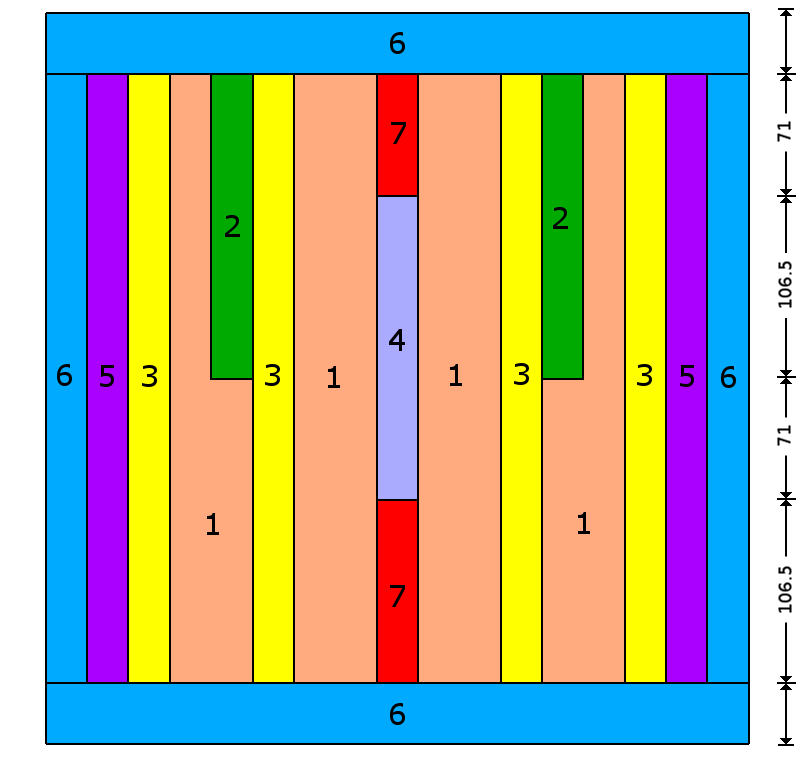
\includegraphics[width=0.75\linewidth] {2.png}
	\caption{Geometrcial model of the VVER-1000 reactor core}
	\label{fig:2}
  \end{center}
\end{figure} 

The test problem for reactor VVER-1000 without reflector   \cite{chao} in two-dimensional approximation 
($\Omega$ is the section of reactor core) is considered. 
The geometrical model of the VVER-1000 reactor core consists of a set of hexagonal assemblies and is presented in Fig. \ref{fig:2}, where the assemblies of various types are marked with various digits. The total size of assembly equals 23.6 cm. Diffusion neutronics constants in the common units are given in Table \ref{t-1}. 
The boundary conditions (\ref{2}) are used at $\gamma_g = 0.5, \ g = 1,2$. 

\begin{table}[h]
\caption{Diffusion neutronics constants for VVER-100}
\label{t-1}
\begin{center}
\begin{tabular}{cccccc}
\rowcolor{col1}
Material & 1 & 2 & 3 & 4 & 5\\
\rowcolor{col3}
$D_1$ & 1.38320e-0 & 1.38299e-0  & 1.39522e-0  & 1.39446e-0  & 1.39506e-0 \\
\rowcolor{col2}
$D_2$ & 3.86277e-1 & 3.89403e-1 & 3.86225e-1 & 3.87723e-1 & 3.84492e-1 \\
\rowcolor{col3}
$\Sigma_{r1}$ & 2.48836e-2 & 2.62865e-2 & 2.45662e-2 & 2.60117e-2 & 2.46141e-2\\
\rowcolor{col2}
$\Sigma_{r2}$ & 6.73049e-2 & 8.10328e-2 & 8.44801e-1 & 9.89671e-2 & 8.93878e-2\\
\rowcolor{col3}
$\Sigma_{s,1\rightarrow 2}$ & 1.64977e-2 & 1.47315e-2 & 1.56219e-2 & 1.40185e-2 & 1.54981e-2\\
\rowcolor{col2}
$\nu\Sigma_{f1}$ & 4.81619e-3 & 4.66953e-3 & 6.04889e-3 & 5.91507e-3 & 6.40256e-3\\
\rowcolor{col3}
$\nu\Sigma_{f2}$ & 8.46154e-2 & 8.52264e-2 & 1.19428e-1 & 1.20497e-1 & 1.29281e-1\\
\end{tabular}
\end{center}
\end{table}

\subsubsection{Solution of Lambda Modes spectral problem} 
The results of solution of the spectral problem (\ref{17})  for the first eigenvalues $k_n = 1 / \lambda_n^{(k)}, \ n = 1,2, ..., 5, \ \lambda_1^{(k)} \leq \lambda_2^{(k)} \leq ...$ 
using the different grids and finite elements are shown in Table \ref{t-2}. These data demonstrate the convergence of approximate computed eigenvalues as the computational grid crowds and degree of the approximating polynomials increases --- $h-p$ finite element method \cite{vidal2014solution}.

\begin{table}[h]
\caption{The eigenvalues $k_n = 1 / \lambda_n^{(k)}, \ n = 1,2, ..., 5$}
\label{t-2}
\begin{center}
\begin{tabular}{ccccc}
\rowcolor{col1}
$\kappa$ & $p$ & $k_1$ &  $k_2, k_3$ &  $k_4,k_5$ \\ 
\rowcolor{col3}
   & 1 & 1.00483 & 0.99272 $\pm$ 1.12018e-06$i$  & 0.97055 $\pm$ 1.18100e-06$i$  \\
\rowcolor{col2}
 6 & 2 & 1.00640 & 0.99473 $\pm$ 1.31480e-06$i$  & 0.97362 $\pm$ 2.49505e-06$i$  \\
\rowcolor{col1}
   & 3 & 1.00645 & 0.99481 $\pm$ 1.52505e-06$i$  & 0.97376 $\pm$ 2.89368e-06$i$  \\
\rowcolor{col3}
   & 1 & 1.00600 & 0.99422 $\pm$ 1.55055e-06$i$  & 0.97285 $\pm$ 2.95842e-06$i$  \\
\rowcolor{col2}
24 & 2 & 1.00645 & 0.99480 $\pm$ 1.51144e-06$i$  & 0.97376 $\pm$ 2.87450e-06$i$  \\
\rowcolor{col1}
   & 3 & 1.00634 & 0.99482 $\pm$ 1.51566e-06$i$  & 0.97377 $\pm$ 2.88024e-06$i$  \\
\rowcolor{col3}
   & 1 & 1.00645 & 0.99466 $\pm$ 1.52518e-06$i$  & 0.97353 $\pm$ 2.90209e-06$i$  \\
\rowcolor{col2}
96 & 2 & 1.00645 & 0.99482 $\pm$ 1.51541e-06$i$  & 0.97377 $\pm$ 2.87990e-06$i$  \\
\rowcolor{col1}
   & 3 & 1.00646 & 0.99482 $\pm$ 1.51558e-06$i$  & 0.97378 $\pm$ 2.88002e-06$i$  \\
\end{tabular}
\end{center}
\end{table}

\begin{figure}[!h]
  \begin{center}
\begin{minipage}{0.49\linewidth}
\center{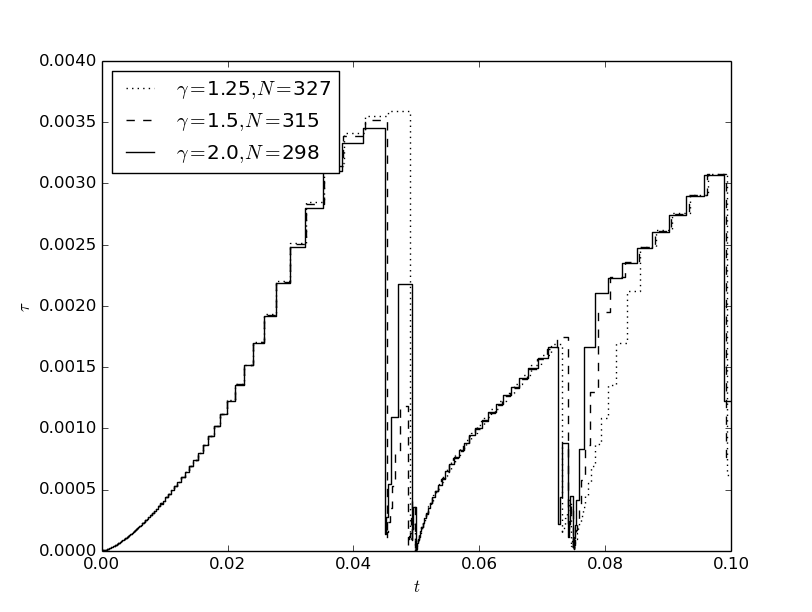
\includegraphics[width=1\linewidth]{3-1.png}} \\
\end{minipage}
\hfill
\begin{minipage}{0.49\linewidth}
\center{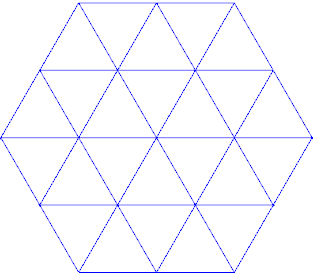
\includegraphics[width=1\linewidth]{3-2.png}} \\
\end{minipage}
\caption{The eigenfunctions $\varphi^{(1)}_1$ (left) and $\varphi^{(1)}_2$ (right).}
\label{fig:3}
  \end{center}
\end{figure}
\begin{figure}[!h]
  \begin{center}
\begin{minipage}{0.49\linewidth}
\center{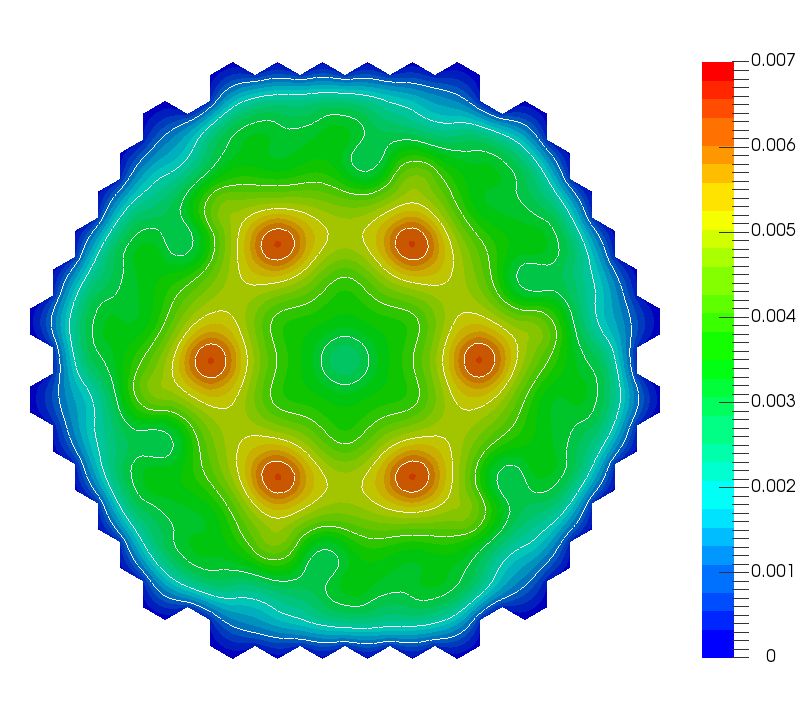
\includegraphics[width=1\linewidth]{4-1.png}} \\
\end{minipage}
\hfill
\begin{minipage}{0.49\linewidth}
\center{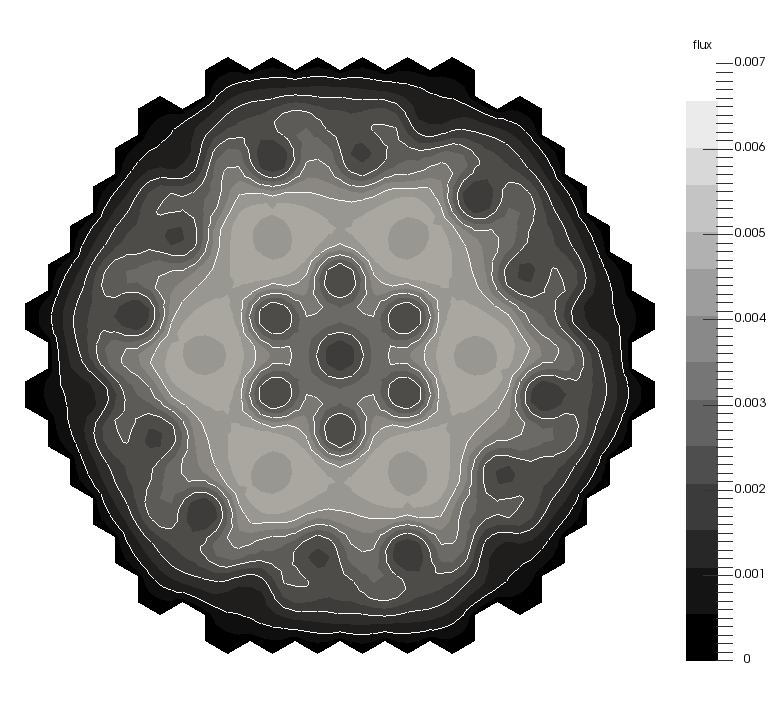
\includegraphics[width=1\linewidth]{4-2.png}} \\
\end{minipage}
\caption{Real part of eigenfunctions $\varphi^{(2)}_1, \ \varphi^{(3)}_1$ (left) and $\varphi^{(4)}_1, \ \varphi^{(5)}_1$ (right).}
\label{fig:4}
  \end{center}
\end{figure}
\begin{figure}[!h]
  \begin{center}
\begin{minipage}{0.49\linewidth}
\center{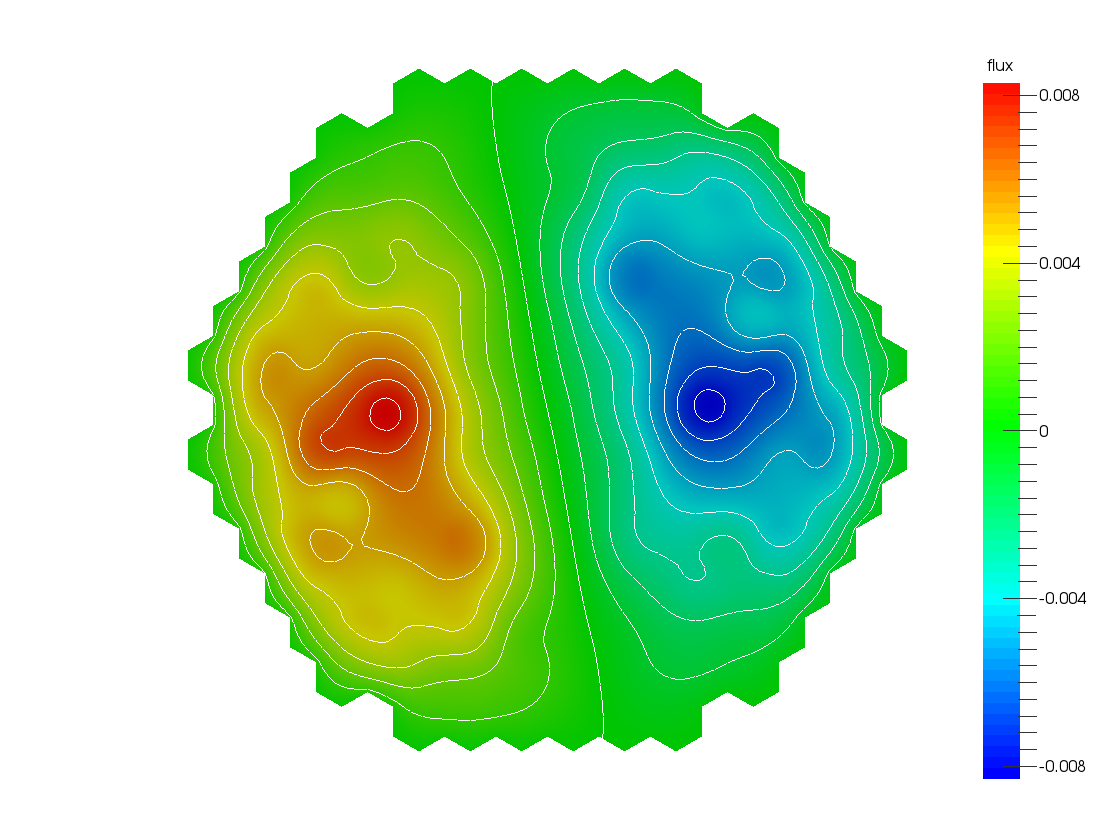
\includegraphics[width=1\linewidth]{5-1.png}} \\
\end{minipage}
\hfill
\begin{minipage}{0.49\linewidth}
\center{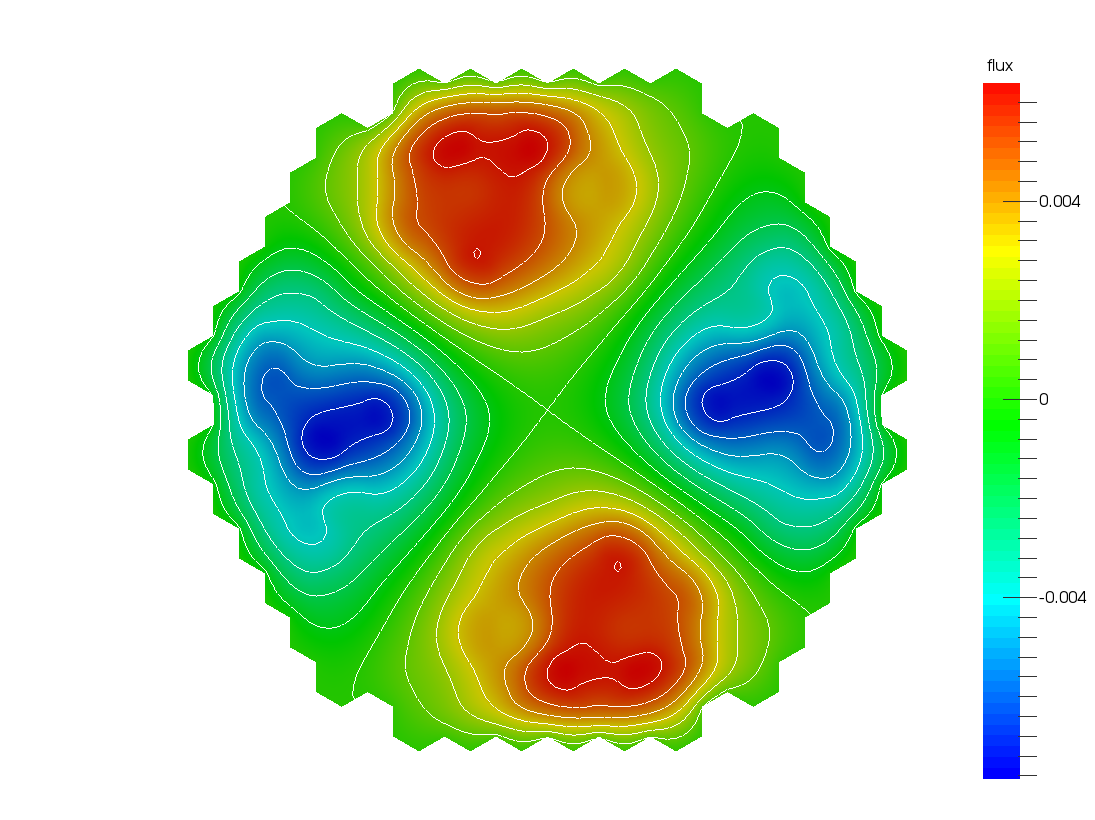
\includegraphics[width=1\linewidth]{5-2.png}} \\
\end{minipage}
\caption{Imaginary part of eigenfunctions $\varphi^{(2)}_1, \ - \varphi^{(3)}_1$ (left) and $\varphi^{(4)}_1, \ - \varphi^{(5)}_1$ (right).}
\label{fig:5}
  \end{center}
\end{figure}
\begin{figure}[!h]
  \begin{center}
\begin{minipage}{0.49\linewidth}
\center{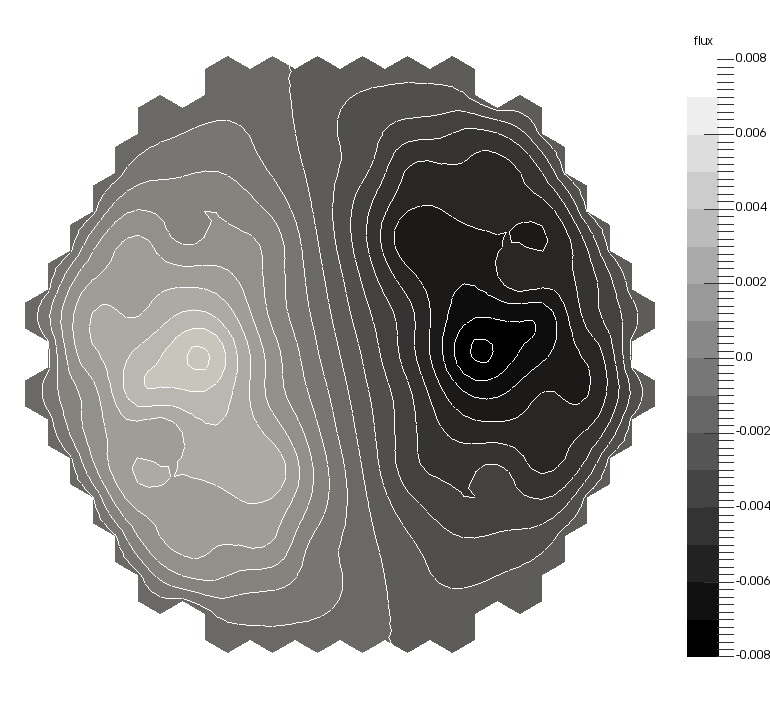
\includegraphics[width=1\linewidth]{6-1.png}} \\
\end{minipage}
\hfill
\begin{minipage}{0.49\linewidth}
\center{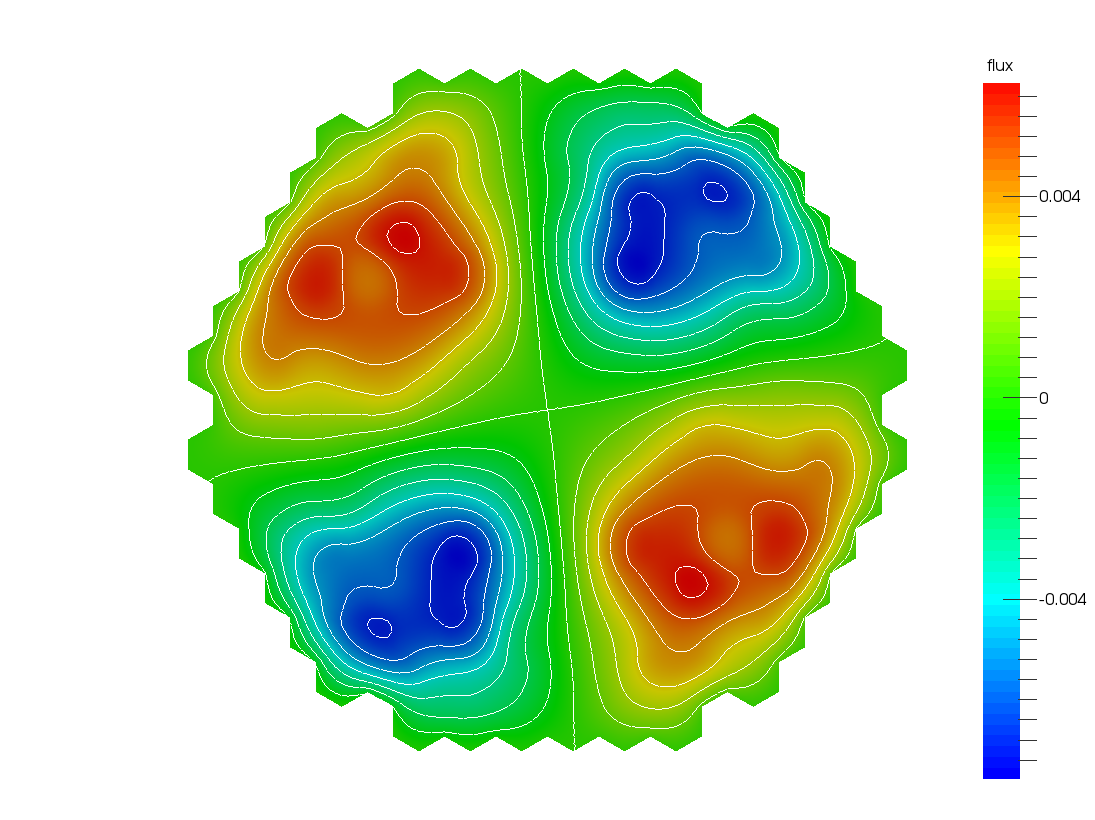
\includegraphics[width=1\linewidth]{6-2.png}} \\
\end{minipage}
\caption{The eigenfunctions $\varphi^{(6)}_1$ (left) and $\varphi^{(7)}_1$ (right).}
\label{fig:6}
  \end{center}
\end{figure}

For the test under consideration, the eigenvalues $k_2, k_3$, $k_4, k_5$ , $k_9, k_{10}$ 
of the spectral problem (\ref{9}) are the complex values with small imaginary parts, and the eigenvalues $k_1, k_6$, $k_7, k_8$ are the real values.
Below we give the graphs of real and imaginary parts of $\bm \varphi^{(n)}$ eigenfunctions which correspond to the first eigenvalues $k_n, \ n = 1, 2, ..., 5$. 
They were calculated using a computational grid with 96 triangles for one assembly and the finite elements of the third degree. The eigenfunctions are normalized so that the norm of real or imaginary part is equal to 1, for example:
\[
 \|\mathrm{Re} \ \varphi^{(n)}_g\| = 1, \quad g = 1,2. 
\] 

The eigenfunctions for fundamental eigenvalue ($n=1$) are shown in the Figure \ref{fig:3}.
The real part of the eigenfunctions $\varphi^{(n)}_1, \ n = 2,3,4,5$ is shown in the Figure \ref{fig:4}.
Figure \ref{fig:5} shows the imaginary part of the eigenfunctions. Figure \ref{fig:6} shows the eigenfunctions $\varphi^{(6)}_1$ at $k_6 \approx  0.95520$ and $\varphi^{(7)}_1$ at $k_7 \approx  0.94838$.



\subsubsection{Solution of Alpha Modes spectral problem} 
\begin{table}[h]
\caption{The eigenvalues $\alpha_n = \lambda_n^{(\alpha )}, \ n = 1,2, ..., 5$}
\label{t-3}
\begin{center}
\begin{tabular}{ccccc}
\rowcolor{col1}
$\kappa$ & $p$ & $\alpha_1$ &  $\alpha_2, \alpha_3$ &  $\alpha_4, \alpha_5$ \\ 
\rowcolor{col3}
   & 1 & -105.032 & 159.802 $\pm$ 0.025510$i$  & 659.109 $\pm$ 0.034667$i$  \\
\rowcolor{col2}
6  & 2 & -139.090 & 115.793 $\pm$ 0.029186$i$  & 591.782 $\pm$ 0.034667$i$  \\
\rowcolor{col1}
   & 3 & -140.223 & 114.035 $\pm$ 0.033814$i$  & 588.762 $\pm$ 0.069025$i$  \\
\rowcolor{col3}
   & 1 & -130.422 & 126.984 $\pm$ 0.034409$i$  & 608.734 $\pm$ 0.070724$i$  \\
\rowcolor{col2}
24 & 2 & -140.187 & 114.089 $\pm$ 0.033512$i$  & 588.849 $\pm$ 0.068555$i$  \\
\rowcolor{col1}
   & 3 & -140.281 & 113.887 $\pm$ 0.033604$i$  & 588.415 $\pm$ 0.068695$i$  \\
\rowcolor{col3}
   & 1 & -137.704 & 117.345 $\pm$ 0.033823$i$  & 593.818 $\pm$ 0.069254$i$  \\
\rowcolor{col2}
96 & 2 & -140.284 & 113.886 $\pm$ 0.033599$i$  & 588.419 $\pm$ 0.068687$i$  \\
\rowcolor{col1}
   & 3 & -140.308 & 113.842 $\pm$ 0.033603$i$  & 588.336 $\pm$ 0.068690$i$  \\
\end{tabular}
\end{center}
\end{table}

The problem  (\ref{18}) is solved at $v_1 = 12 500 000$ and $v_2 = 250 000$. The results of solution of the spectral problem (\ref{18}) for the first eigenvalues $\alpha_n = \lambda_n^{(\alpha)}, \ n = 1,2, ..., 5, \  \lambda_1^{(\alpha)} \leq  \lambda_2^{(\alpha )} \leq ...$
at different computational grids using different finite-element approximations are shown in Table \ref{t-3}. 
The eigenvalues $\alpha_2, \alpha_3$, $\alpha_4, \alpha_5$, $\alpha_9, \alpha_{10}$ of the spectral problem (\ref{10}), like for the spectral problem (\ref{9}), are the complex values with small imaginary parts, and the eigenvalues $\alpha_1, \alpha_6$, $\alpha_7, \alpha_8$ are the real values.
\begin{figure}[h]
  \begin{center}
\begin{minipage}{0.49\linewidth}
\center{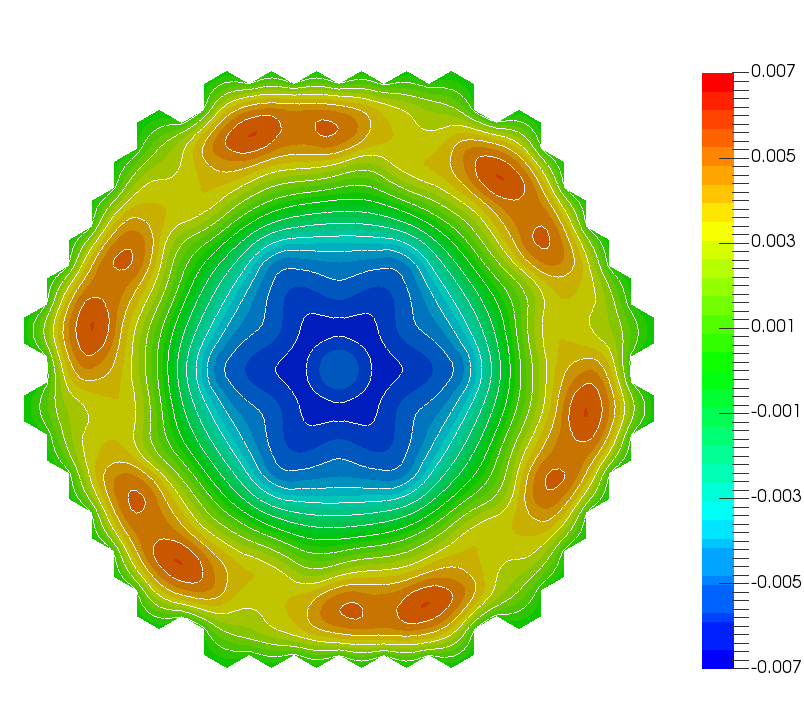
\includegraphics[width=1\linewidth]{7-1.png}} \\
\end{minipage}
\hfill
\begin{minipage}{0.49\linewidth}
\center{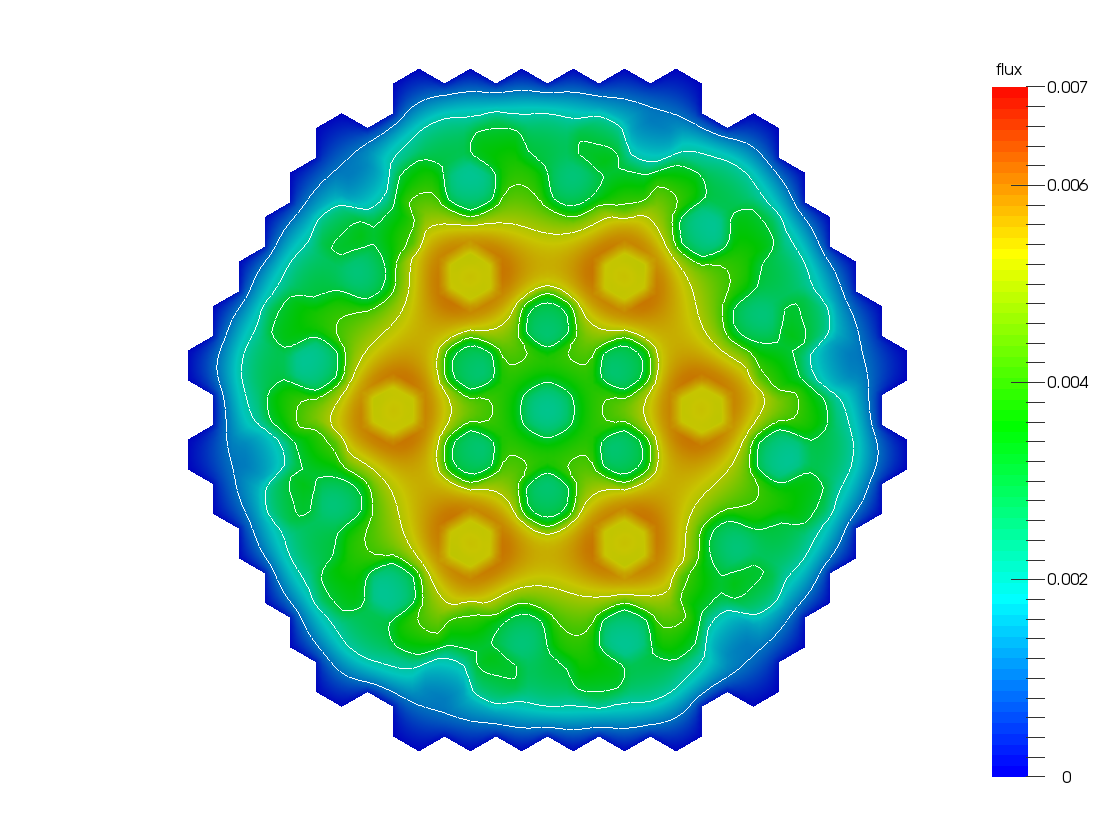
\includegraphics[width=1\linewidth]{7-2.png}} \\
\end{minipage}
\caption{The eigenfunctions $\varphi^{(1)}_1$ (left) and $\varphi^{(1)}_2$ (right).}
\label{fig:7}
  \end{center}
\end{figure}
\begin{figure}[h]
  \begin{center}
\begin{minipage}{0.49\linewidth}
\center{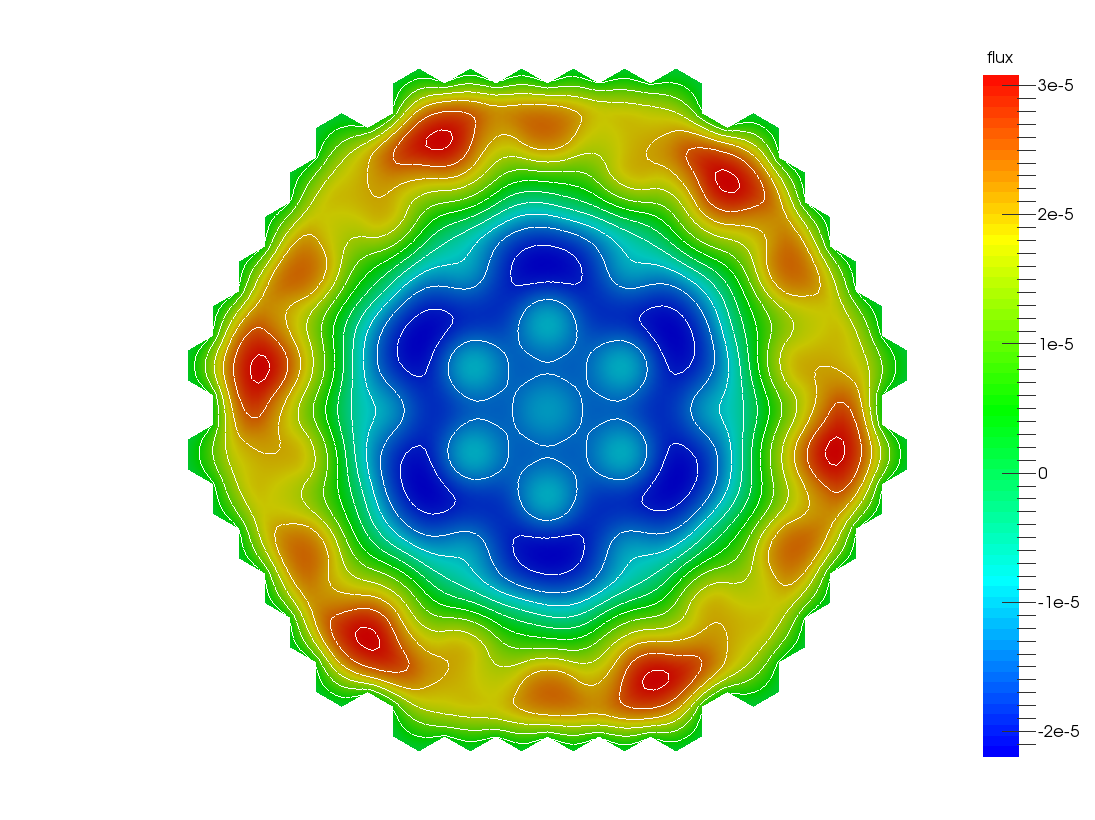
\includegraphics[width=1\linewidth]{8-1.png}} \\
\end{minipage}
\hfill
\begin{minipage}{0.49\linewidth}
\center{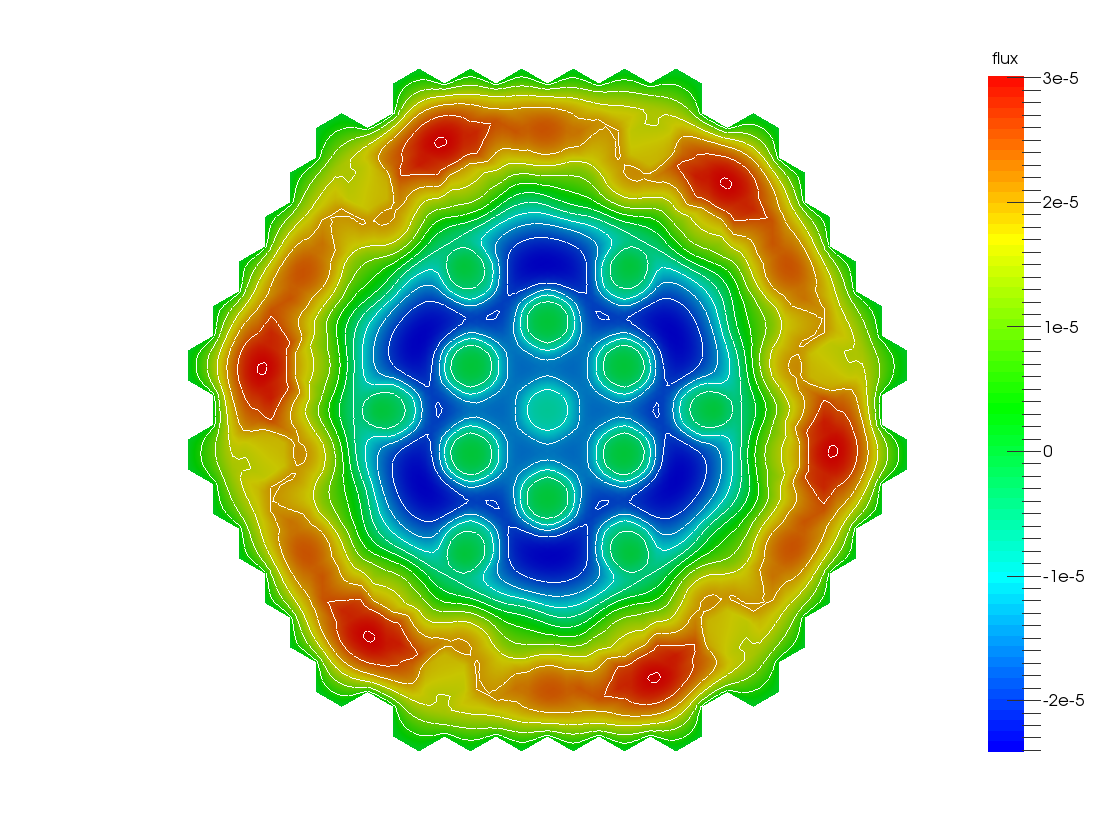
\includegraphics[width=1\linewidth]{8-2.png}} \\
\end{minipage}
\caption{Difference of eigenfunctions $\delta \varphi^{(1)}_1$ (left) and $\delta \varphi^{(1)}_2$ (right).}
\label{fig:8}
  \end{center}
\end{figure}
\begin{figure}[!h]
  \begin{center}
\begin{minipage}{0.49\linewidth}
\center{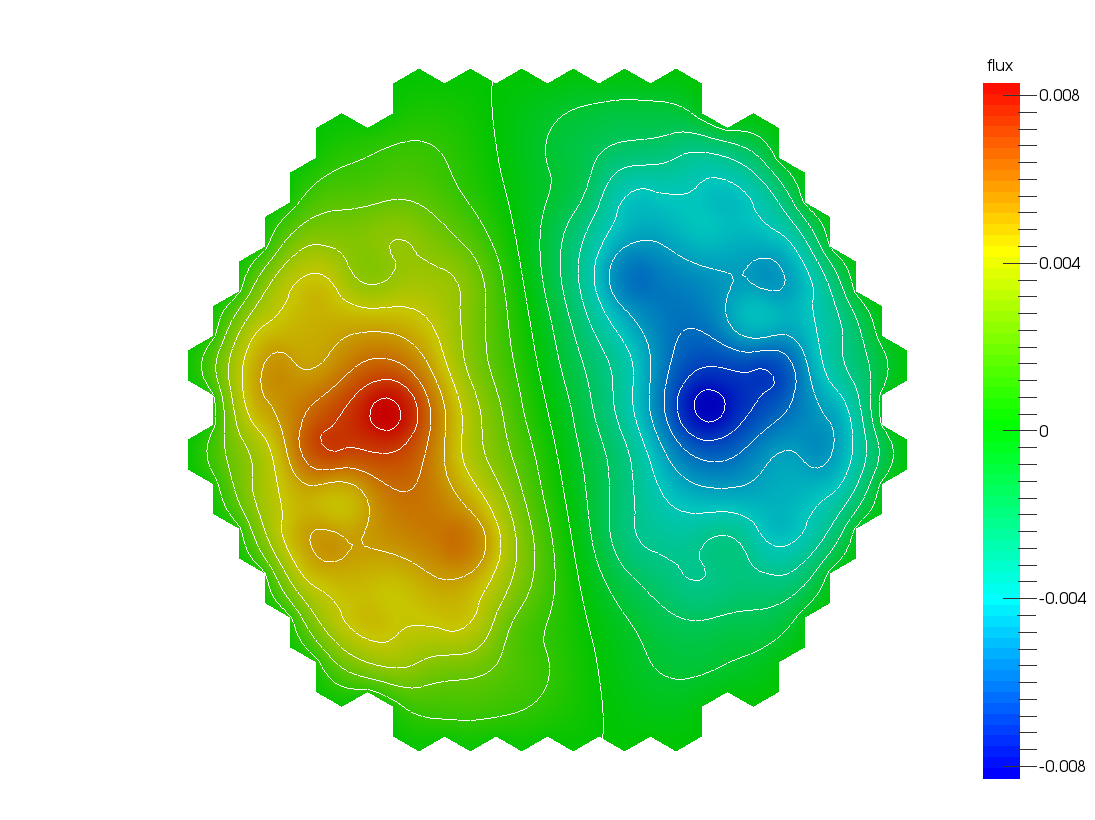
\includegraphics[width=1\linewidth]{9-1.png}} \\
\end{minipage}
\hfill
\begin{minipage}{0.49\linewidth}
\center{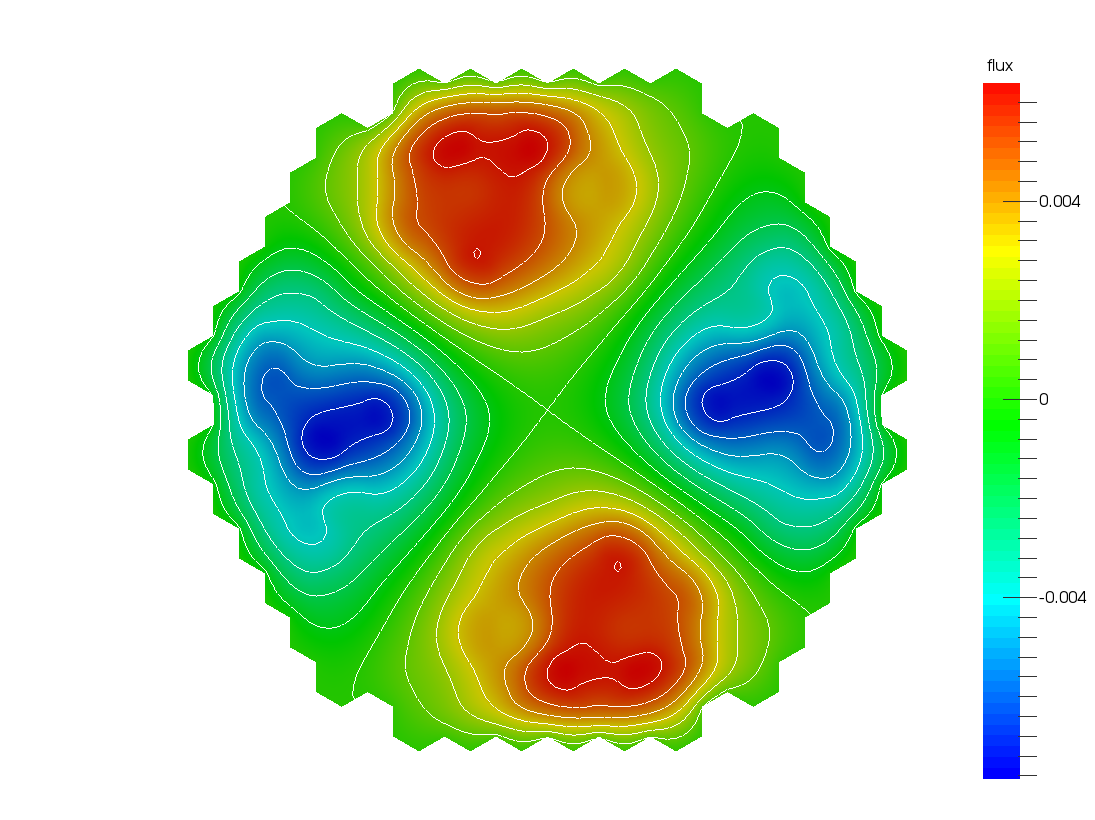
\includegraphics[width=1\linewidth]{9-2.png}} \\
\end{minipage}
\caption{Real part of eigenfunctions $\varphi^{(2)}_1, \ \varphi^{(3)}_1$ (left) and $\varphi^{(4)}_1, \ \varphi^{(5)}_1$ (right).}
\label{fig:9}
  \end{center}
\end{figure}
\begin{figure}[!h]
  \begin{center}
\begin{minipage}{0.49\linewidth}
\center{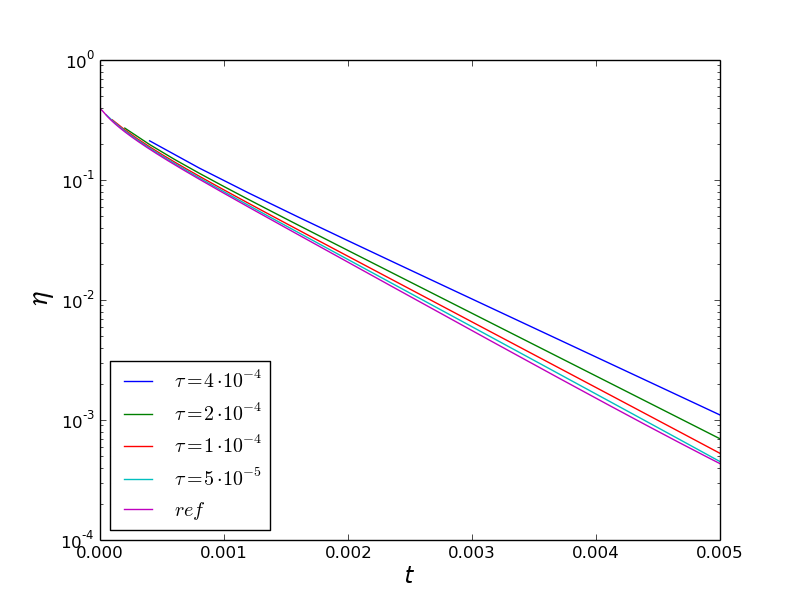
\includegraphics[width=1\linewidth]{10-1.png}} \\
\end{minipage}
\hfill
\begin{minipage}{0.49\linewidth}
\center{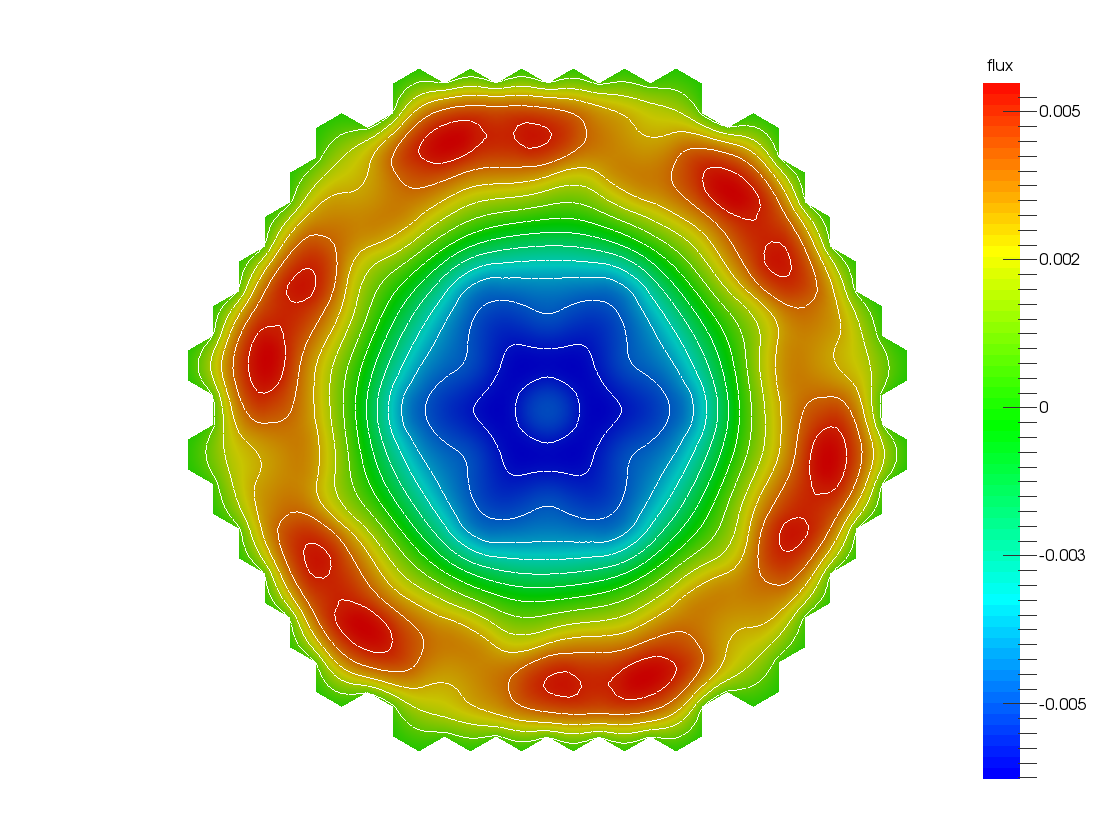
\includegraphics[width=1\linewidth]{10-2.png}} \\
\end{minipage}
\caption{Imaginary part of eigenfunctions $\varphi^{(2)}_1, \ - \varphi^{(3)}_1$ (left) and $\varphi^{(4)}_1, \ - \varphi^{(5)}_1$ (right).}
\label{fig:10}
  \end{center}
\end{figure}
\begin{figure}[!h]
  \begin{center}
\begin{minipage}{0.49\linewidth}
\center{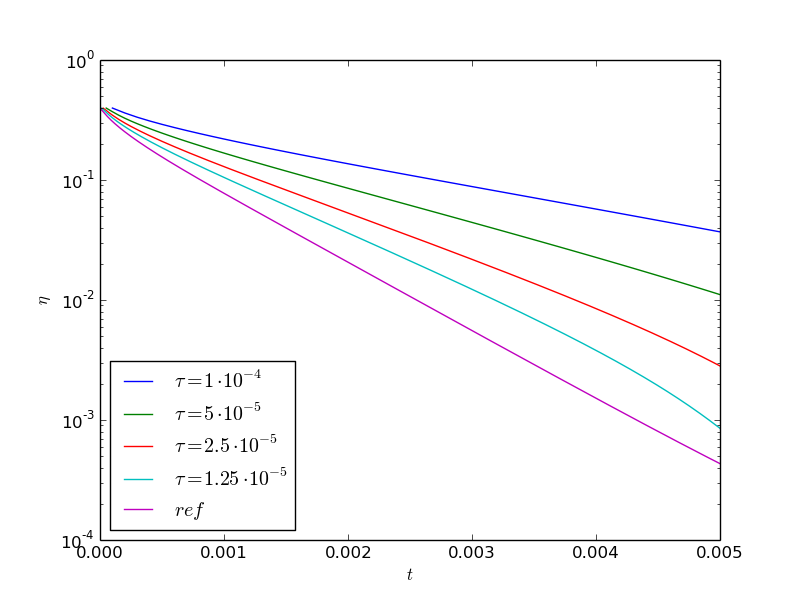
\includegraphics[width=1\linewidth]{11-1.png}} \\
\end{minipage}
\hfill
\begin{minipage}{0.49\linewidth}
\center{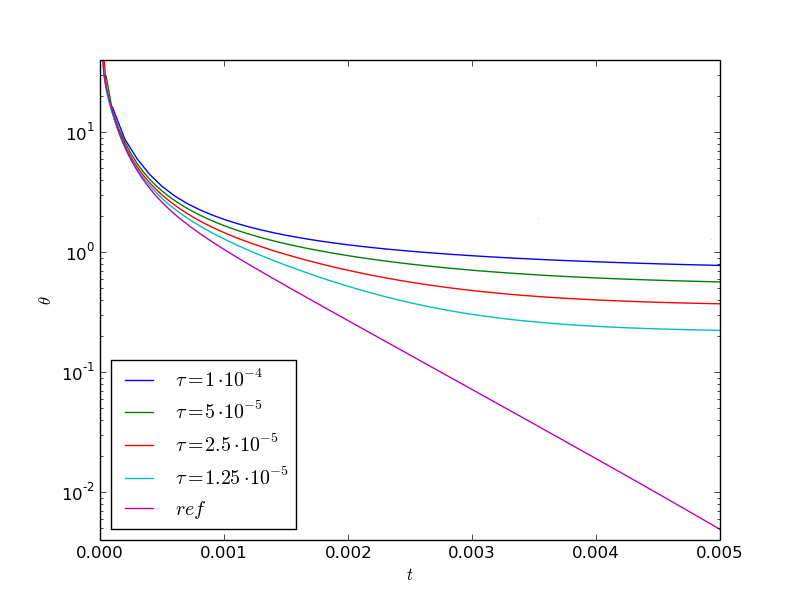
\includegraphics[width=1\linewidth]{11-2.png}} \\
\end{minipage}
\caption{The eigenfunctions $\varphi^{(6)}_1$ (left) and $\varphi^{(7)}_1$ (right).}
\label{fig:11}
  \end{center}
\end{figure}

The eigenfunctions for fundamental eigenvalue ($n=1$) of the spectral problem (\ref{18}) are shown in the Fig. \ref{fig:7}. Due to the fact that a state of the reactor is close to critical ($k = k_1 \approx  1.00646$), the fundamental eigenfunctions of the spectral problem (\ref{17}) are close to the fundamental eigenfunctions of the spectral problem (\ref{18}).
Figure \ref{fig:8} shows the difference of $\alpha$-eigenfunction and $\lambda$-eigenfunction.  


The real part of the eigenfunctions $\varphi^{(n)}_1, \ n = 2,3,4,5$ is shown in the Figure \ref{fig:9}.
Figure \ref{fig:10} shows the imaginary part of these eigenfunctions.
Figure \ref{fig:11} shows the eigenfunctions $\varphi^{(6)}_1$ at $\alpha_6 \approx  1028.440$ and 
$\varphi^{(7)}_1$ at $\alpha_7 \approx  1180.547$.

The first eigenfunctions of the problems (\ref{17}) and (\ref{18}) are close to each other in topology.
The eigenvalues $\lambda_1^{(\alpha)} \leq  \lambda_2^{(\alpha)} \leq ...$
are well separated. In our example, the fundamental eigenvalue is negative and therefore the main harmonic will increase, while all others will attenuate. A regular mode of the reactor is thereby defined. The value $\alpha = \lambda_1^{(\alpha)}$ determines the amplitude of neutron field development and connects directly with reactor period in the regular mode.

\subsubsection{Solution of Delta  Modes spectral problem} 
The results of solution of this spectral problem for the first five eigenvalues are shown in Table \ref{t-4}. All the eigenvalues are real, and the value $\delta = \delta_1 \approx -22991.05$ is far enough from the value $\alpha  = \alpha_1 \approx -140.308$.
The eigenvalues of the problem (\ref{19}) are of little importance. Therefore only $\varphi^{(1)}_1$ and $\varphi^{(2)}_1$ are given in Figure \ref{fig:12}.
\begin{table}[h]
\caption{The eigenfunctions $\delta_n = 1 / \lambda_n^{(\delta )}, \ n = 1,2,...,5$}
\label{t-4}
\begin{center}
\begin{tabular}{ccccccc}
\rowcolor{col1}
$\kappa$ & $p$ & $\delta_1$ &  $\delta_2$ &  $\delta_3$ &  $\delta_4$ &  $\delta_5$ \\ 
\rowcolor{col3}
   & 1 & -22170.12 & -22058.40 & -22058.39 & -21768.84 & -21768.82 \\
\rowcolor{col2}
6  & 2 & -22933.98 & -22830.17 & -22830.16 & -22563.69 & -22563.67 \\
\rowcolor{col1}
   & 3 & -22982.60 & -22878.57 & -22878.56 & -22611.14 & -22611.12 \\
\rowcolor{col3}
   & 1 & -22745.06 & -22639.74 & -22639.73 & -22369.01 & -22368.99 \\
\rowcolor{col2}
24 & 2 & -22923.50 & -22819.17 & -22819.17 & -22551.00 & -22550.98 \\
\rowcolor{col1}
   & 3 & -22989.87 & -22885.85 & -22885.84 & -22618.47 & -22618.44 \\
\rowcolor{col3}
   & 1 & -22923.50 & -22819.17 & -22819.17 & -22551.00 & -22550.98 \\
\rowcolor{col2}
96 & 2 & -22989.61 & -22885.60 & -22885.59 & -22618.22 & -22618.20 \\
\rowcolor{col1}
   & 3 & -22991.05 & -22887.04 & -22887.03 & -22619.66 & -22619.63 \\
\end{tabular}
\end{center}
\end{table}
\begin{figure}[h]
  \begin{center}
\begin{minipage}{0.49\linewidth}
\center{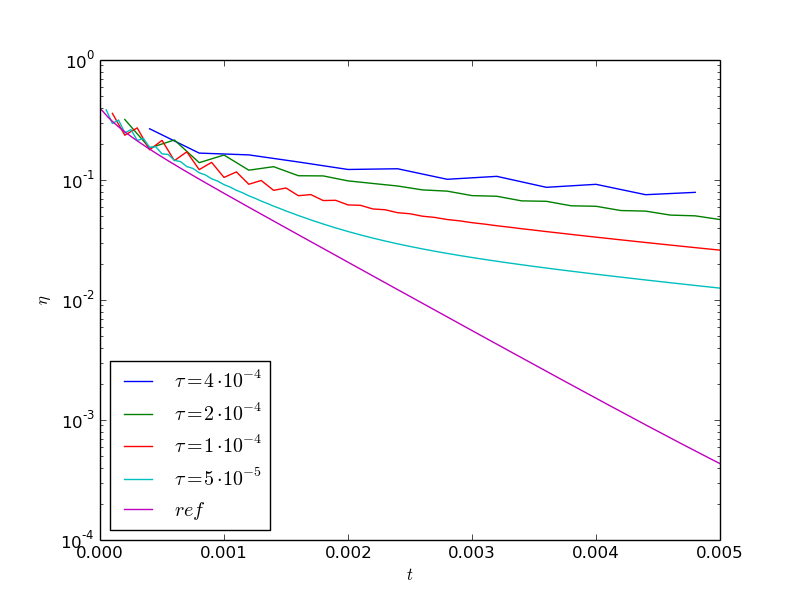
\includegraphics[width=1\linewidth]{12-1.png}} \\
\end{minipage}
\hfill
\begin{minipage}{0.49\linewidth}
\center{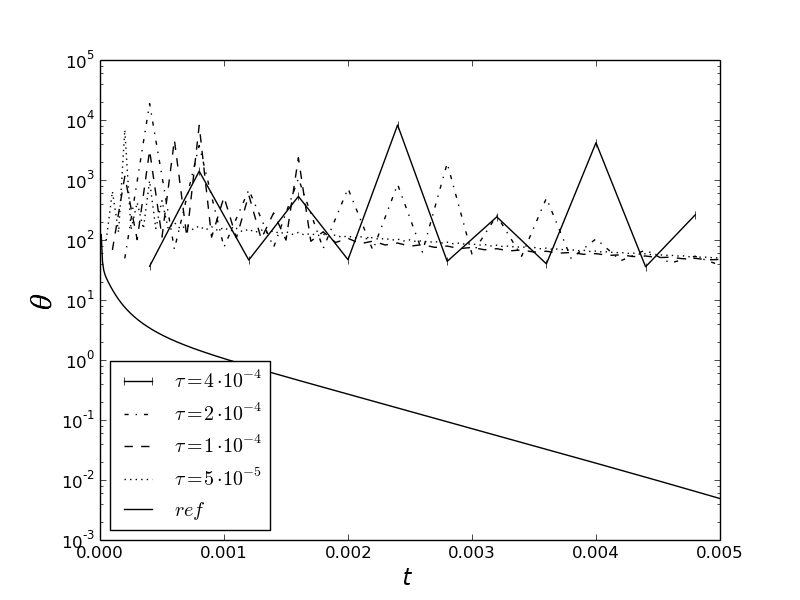
\includegraphics[width=1\linewidth]{12-2.png}} \\
\end{minipage}
\caption{The eigenfunctions $\varphi^{(1)}_1$ (left) and $\varphi^{(2)}_1$ (right).}
\label{fig:12}
  \end{center}
\end{figure}

\subsection{HWR problem}
This benchmark simulate the active zone of a large heavy-water reactor HWR \cite{chao}. The geometrical model of the HWR reactor core consists of a set of hexagonal assemblies and is presented in Fig. \ref{fig:13}. The total size of assembly equals 17.78 cm. Diffusion neutronics constants in the common units are given in Table \ref{t-5}. 
The boundary conditions (\ref{2}) are used at $\gamma_g = 0.5, \ g = 1,2$. 
\begin{table}[!h]
\small
\caption{Diffusion neutronics constants for HWR}
\label{t-5}
\begin{center}
\begin{tabular}{cccccc}
\rowcolor{col1}
Material & Group & $D$ & $\Sigma_r$ & $\Sigma_{1\to 2}$ & $\nu\Sigma_f$\\
\rowcolor{col3}
1 & 1 & 1.38250058 & 1.1105805e-2 & 8.16457e-3 & 2.26216e-3 \\
\rowcolor{col2}
  & 2 & 0.89752185 & 2.2306487e-2 &            & 2.30623e-2 \\
\rowcolor{col3}
2 & 1 & 1.38255219 & 1.1174585e-2 & 8.22378e-3 & 2.22750e-3 \\
\rowcolor{col2}
  & 2 & 0.89749043 & 2.2387609e-2 &            & 2.26849e-2 \\
\rowcolor{col3}
3 & 1 & 1.37441741 & 1.0620368e-2 & 8.08816e-3 & 2.14281e-3 \\
\rowcolor{col2}
  & 2 & 0.88836771 & 1.6946527e-2 &            & 2.04887e-2 \\
\rowcolor{col3}
4 & 1 & 1.31197955 & 1.2687953e-2 & 1.23115e-2 & 0.0 \\
\rowcolor{col2}
  & 2 & 0.87991376 & 5.2900925e-2 &            & 0.0 \\
\rowcolor{col3}
6 & 1 & 1.38138909 & 1.056312e-2 & 7.76568e-3 & 2.39469e-3 \\
\rowcolor{col2}
  & 2 & 0.90367052 & 2.190298e-2 &            & 2.66211e-2 \\
\rowcolor{col3}
7 & 1 & 1.30599110 & 1.1731321e-2 & 1.10975e-2 & 0.0 \\
\rowcolor{col2}
  & 2 & 0.83725587 & 4.3330365e-3 &            & 0.0 \\
\rowcolor{col3}
8 & 1 & 1.29192957 & 1.1915316e-2 & 1.15582e-2 & 0.0 \\
\rowcolor{col2}
  & 2 & 0.81934103 & 3.0056488e-4 &            & 0.0 \\
\rowcolor{col3}
9 & 1 & 1.06509884 & 2.8346221e-2 & 2.61980e-2 & 0.0 \\
\rowcolor{col3}
  & 2 & 0.32282849 & 3.3348874e-2 &            & 0.0 \\  
\end{tabular}
\end{center}
\end{table}
\begin{figure}[!h]
  \begin{center}
    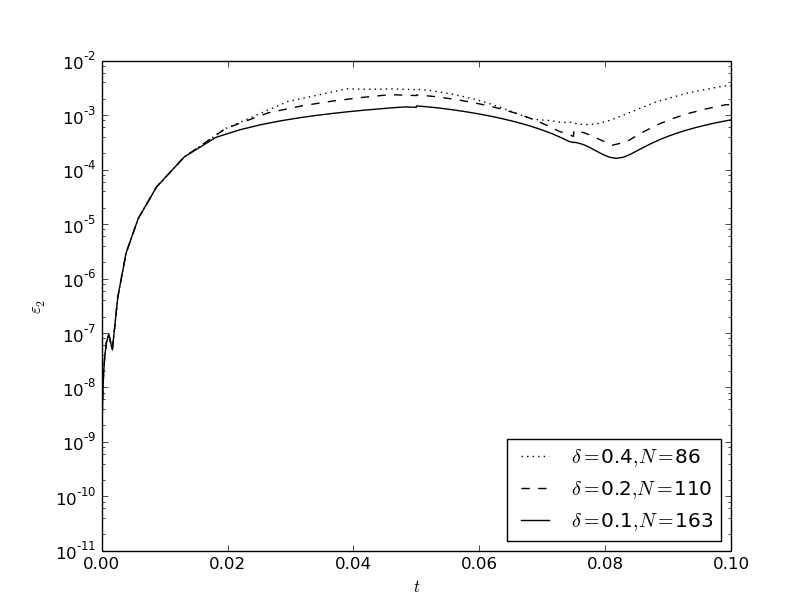
\includegraphics[width=0.75\linewidth] {13.png}
	\caption{Geometrcial model of the HWR reactor core}
	\label{fig:13}
  \end{center}
\end{figure} 

\subsubsection{Solution of Lambda Modes spectral problem}
The results of solution of the spectral problem (\ref{17})  for the first eigenvalues $k_n = 1 / \lambda_n^{(k)}, \ n = 1,2, ..., 5, \ \lambda_1^{(k)} \leq \lambda_2^{(k)} \leq ...$ 
using the different grids and finite elements are shown in Table \ref{t-6}. These data demonstrate the convergence of approximate computed eigenvalues as the computational grid crowds and degree of the approximating polynomials increases --- $h-p$ finite element method.

\begin{table}[h]
\caption{The eigenvalues $k_n = 1 / \lambda_n^{(k)}, \ n = 1,2, ..., 5$}
\label{t-6}
\begin{center}
\begin{tabular}{ccccc}
\rowcolor{col1}
$\kappa$ & $p$ & $k_1$ &  $k_2, k_3$ &  $k_4,k_5$ \\ 
\rowcolor{col3}
   & 1 & 0.99198 & 0.98360 $\pm$ 1.06467e-05$i$  & 0.96414 $\pm$ 1.96893e-05$i$  \\
\rowcolor{col2}
 6 & 2 & 0.99199 & 0.98362 $\pm$ 1.16182e-05$i$  & 0.96427 $\pm$ 2.15201e-05$i$  \\
\rowcolor{col1}
   & 3 & 0.99196 & 0.98360 $\pm$ 1.16441e-05$i$  & 0.96424 $\pm$ 2.15627e-05$i$  \\
\rowcolor{col3}
   & 1 & 0.99198 & 0.98361 $\pm$ 1.13901e-05$i$  & 0.96423 $\pm$ 2.10911e-05$i$  \\
\rowcolor{col2}
24 & 2 & 0.99197 & 0.98360 $\pm$ 1.16422e-05$i$  & 0.96424 $\pm$ 2.15595e-05$i$  \\
\rowcolor{col1}
   & 3 & 0.99196 & 0.99359 $\pm$ 1.16449e-05$i$  & 0.96424 $\pm$ 2.15643e-05$i$  \\
\rowcolor{col3}
   & 1 & 0.99197 & 0.98360 $\pm$ 1.15799e-05$i$  & 0.96424 $\pm$ 2.14440e-05$i$  \\
\rowcolor{col2}
96 & 2 & 0.99196 & 0.98359 $\pm$ 1.16448e-05$i$  & 0.96424 $\pm$ 2.15640e-05$i$  \\
\rowcolor{col1}
   & 3 & 0.99196 & 0.98359 $\pm$ 1.16447e-05$i$  & 0.96424 $\pm$ 2.15639e-05$i$  \\
\end{tabular}
\end{center}
\end{table}

The eigenvalues $k_2, k_3$, $k_4, k_5$ , $k_9, k_{10}$ 
of the spectral problem (\ref{9}) are the complex values with small imaginary parts, and the eigenvalues $k_1, k_6$, $k_7, k_8$ are the real values.
Below we give the graphs of real and imaginary parts of $\bm \varphi^{(n)}$ eigenfunctions which correspond to the first eigenvalues $k_n, \ n = 1, 2, ..., 5$. 

The eigenfunctions for fundamental eigenvalue ($n=1$) are shown in the Figure \ref{fig:14}.
The real part of the eigenfunctions $\varphi^{(n)}_1, \ n = 2,3,4,5$ is shown in the Figure \ref{fig:15}.
Figure \ref{fig:16} shows the imaginary part of the eigenfunctions.

\begin{figure}[h]
  \begin{center}
\begin{minipage}{0.49\linewidth}
\center{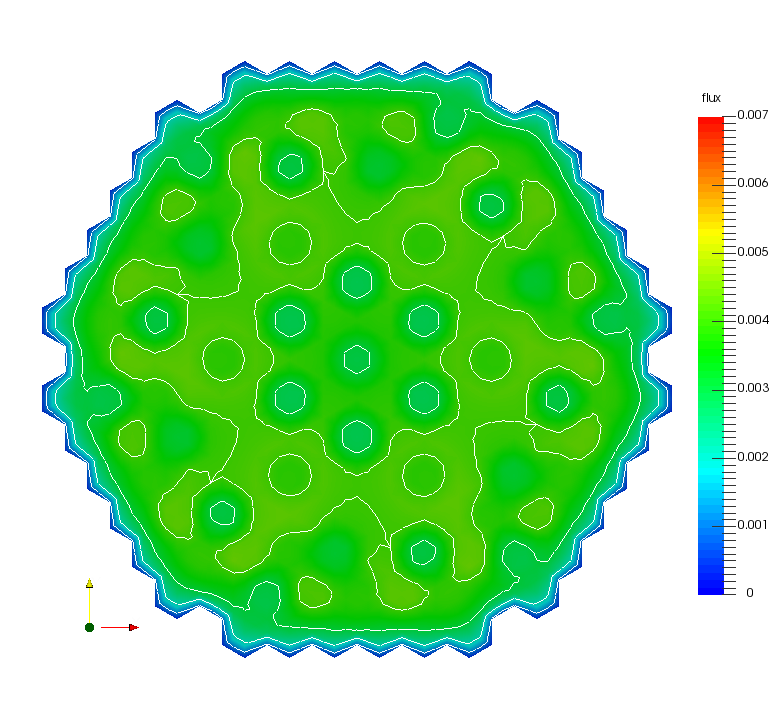
\includegraphics[width=1\linewidth]{14-1.png}} \\
\end{minipage}
\hfill
\begin{minipage}{0.49\linewidth}
\center{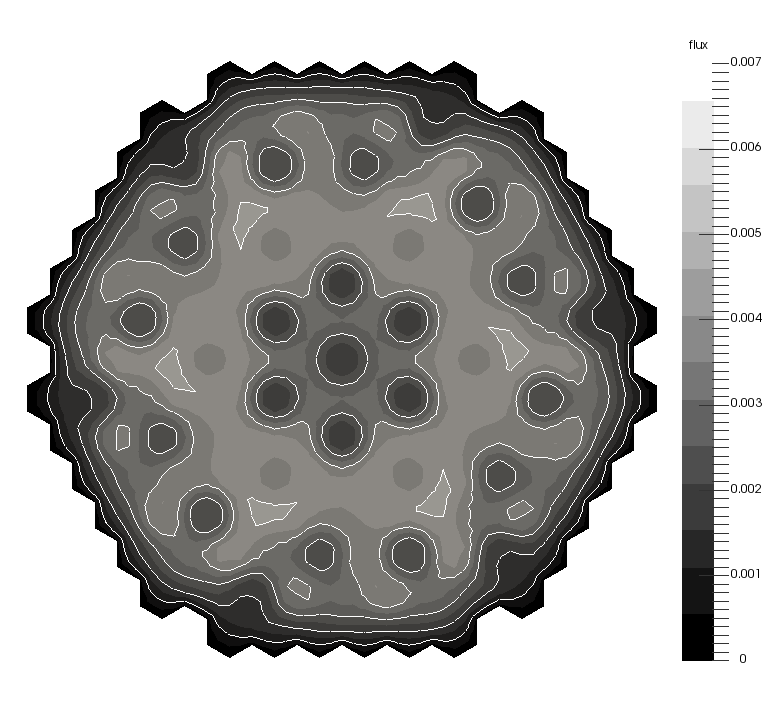
\includegraphics[width=1\linewidth]{14-2.png}} \\
\end{minipage}
\caption{The eigenfunctions $\varphi^{(1)}_1$ (left) and $\varphi^{(1)}_2$ (right).}
\label{fig:14}
  \end{center}
\end{figure}

\begin{figure}[h]
  \begin{center}
\begin{minipage}{0.49\linewidth}
\center{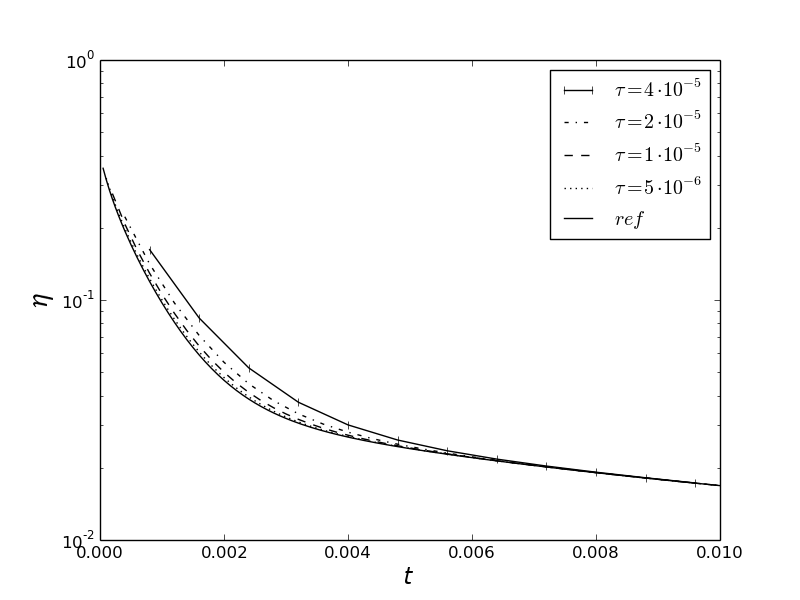
\includegraphics[width=1\linewidth]{15-1.png}} \\
\end{minipage}
\hfill
\begin{minipage}{0.49\linewidth}
\center{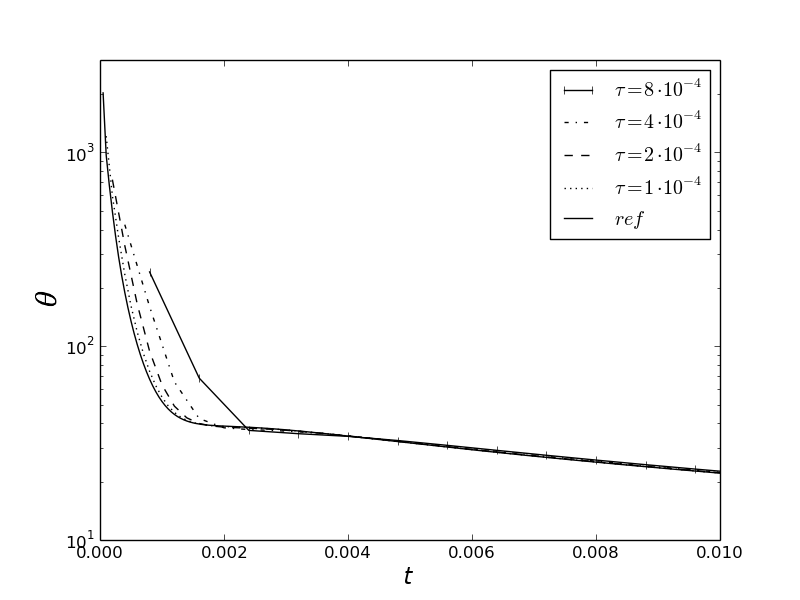
\includegraphics[width=1\linewidth]{15-2.png}} \\
\end{minipage}
\caption{Real part of eigenfunctions $\varphi^{(2)}_1, \ \varphi^{(3)}_1$ (left) and $\varphi^{(4)}_1, \ \varphi^{(5)}_1$ (right).}
\label{fig:15}
  \end{center}
\end{figure}

\begin{figure}[h]
  \begin{center}
\begin{minipage}{0.49\linewidth}
\center{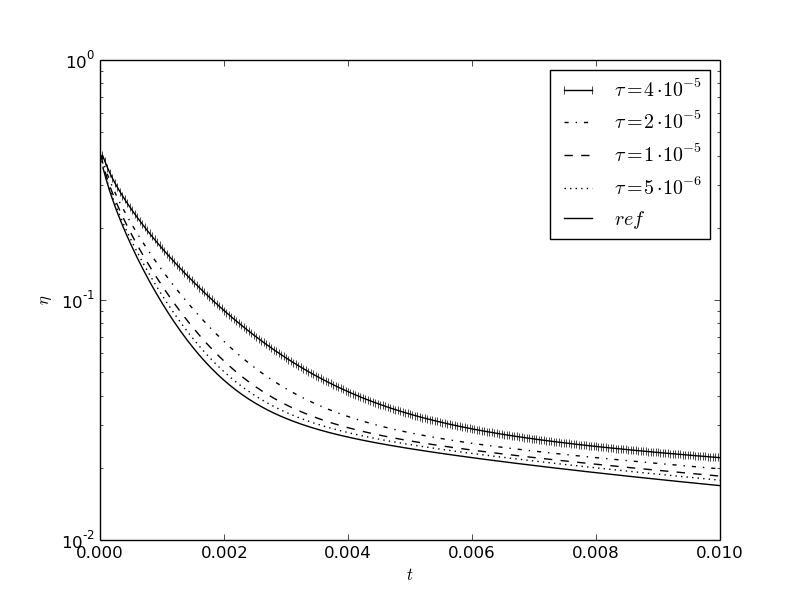
\includegraphics[width=1\linewidth]{16-1.png}} \\
\end{minipage}
\hfill
\begin{minipage}{0.49\linewidth}
\center{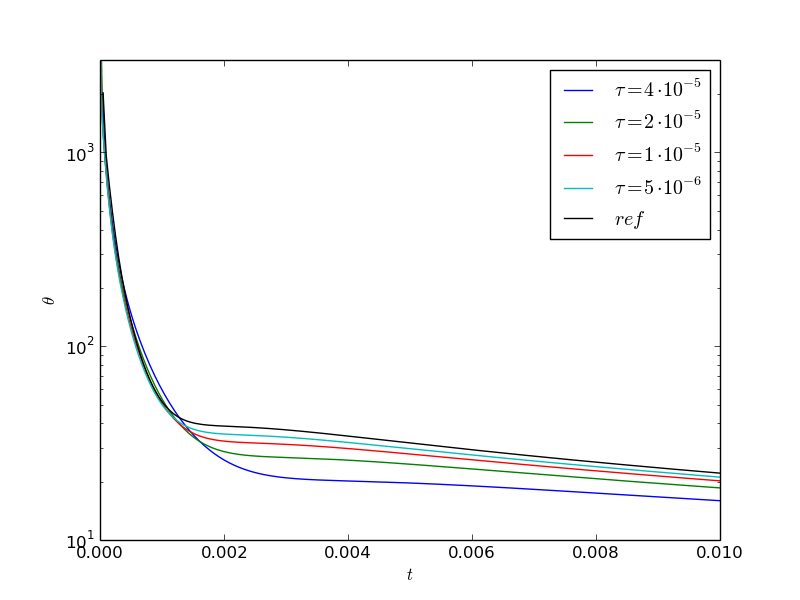
\includegraphics[width=1\linewidth]{16-2.png}} \\
\end{minipage}
\caption{Imaginary part of eigenfunctions $\varphi^{(2)}_1, \ - \varphi^{(3)}_1$ (left) and $\varphi^{(4)}_1, \ - \varphi^{(5)}_1$ (right).}
\label{fig:16}
  \end{center}
\end{figure}

\subsubsection{Solution of Alpha Modes spectral problem} 
The problem  (\ref{18}) is solved at $v_1 = 12 500 000$ and $v_2 = 250 000$. The results of solution of the spectral problem (\ref{18}) for the first eigenvalues $\alpha_n = \lambda_n^{(\alpha)}, \ n = 1,2, ..., 5, \  \lambda_1^{(\alpha)} \leq  \lambda_2^{(\alpha )} \leq ...$
at different computational grids using different finite-element approximations are shown in Table \ref{t-7}. 
The eigenvalues $\alpha_2, \alpha_3$, $\alpha_4, \alpha_5$, $\alpha_9, \alpha_{10}$ of the spectral problem (\ref{10}), like for the spectral problem (\ref{9}), are the complex values with small imaginary parts, and the eigenvalues $\alpha_1, \alpha_6$, $\alpha_7, \alpha_8$ are the real values.

\begin{table}[h]
\caption{The eigenvalues $\alpha_n = \lambda_n^{(\alpha )}, \ n = 1,2, ..., 5$}
\label{t-7}
\begin{center}
\begin{tabular}{ccccc}
\rowcolor{col1}
$\kappa$ & $p$ & $\alpha_1$ &  $\alpha_2, \alpha_3$ &  $\alpha_4, \alpha_5$ \\ 
\rowcolor{col3}
   & 1 & 42.28145 & 85.12917 $\pm$ 0.05604$i$ & 183.97351 $\pm$ 0.10320$i$  \\
\rowcolor{col2}
6  & 2 & 42.13522 & 84.73725 $\pm$ 0.06117$i$  & 182.79517 $\pm$ 0.11345$i$  \\
\rowcolor{col1}
   & 3 & 42.25852 & 84.86342 $\pm$ 0.06130$i$  & 182.91188 $\pm$ 0.11367$i$  \\
\rowcolor{col3}
   & 1 & 42.19593 & 84.86062 $\pm$ 0.05997$i$  & 183.11506 $\pm$ 0.11104$i$  \\
\rowcolor{col2}
24 & 2 & 42.25260 & 84.85735 $\pm$ 0.06129$i$  & 182.90628 $\pm$ 0.11365$i$  \\
\rowcolor{col1}
   & 3 & 42.26300 & 84.86756 $\pm$ 0.06130$i$  & 182.91450 $\pm$ 0.11367$i$  \\
\rowcolor{col3}
   & 1 & 42.24114 & 84.86101 $\pm$ 0.06096$i$  & 182.96129 $\pm$ 0.11301$i$  \\
\rowcolor{col2}
96 & 2 & 42.26235 & 84.86689 $\pm$ 0.06130$i$  & 182.91391 $\pm$ 0.11367$i$  \\
\rowcolor{col1}
   & 3 & 42.26266 & 84.86709 $\pm$ 0.06130$i$  & 182.91375 $\pm$ 0.11367$i$  \\
\end{tabular}
\end{center}
\end{table}
\begin{figure}[!h]
  \begin{center}
\begin{minipage}{0.49\linewidth}
\center{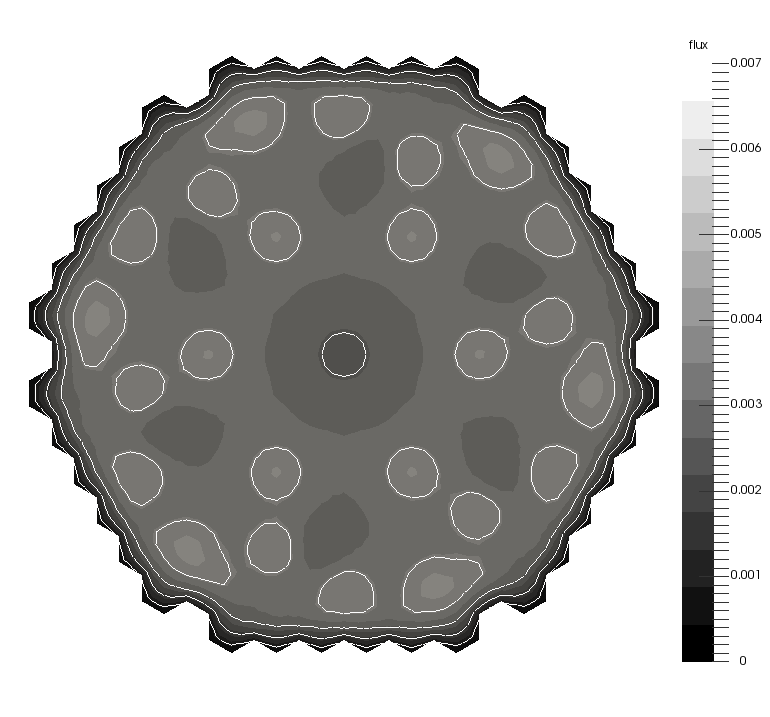
\includegraphics[width=1\linewidth]{17-1.png}} \\
\end{minipage}
\hfill
\begin{minipage}{0.49\linewidth}
\center{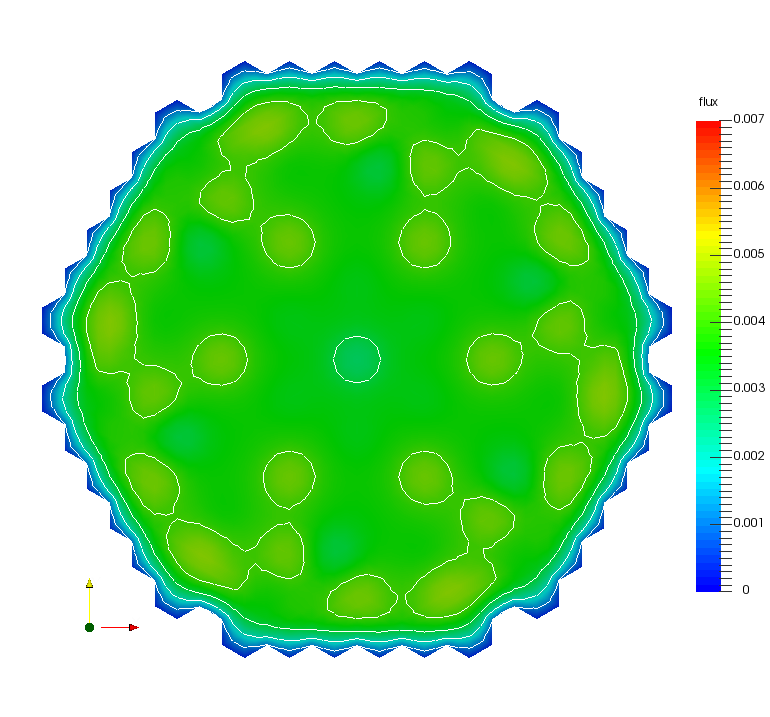
\includegraphics[width=1\linewidth]{17-2.png}} \\
\end{minipage}
\caption{The eigenfunctions $\varphi^{(1)}_1$ (left) and $\varphi^{(1)}_2$ (right).}
\label{fig:17}
  \end{center}
\end{figure}
\begin{figure}[!h]
  \begin{center}
\begin{minipage}{0.49\linewidth}
\center{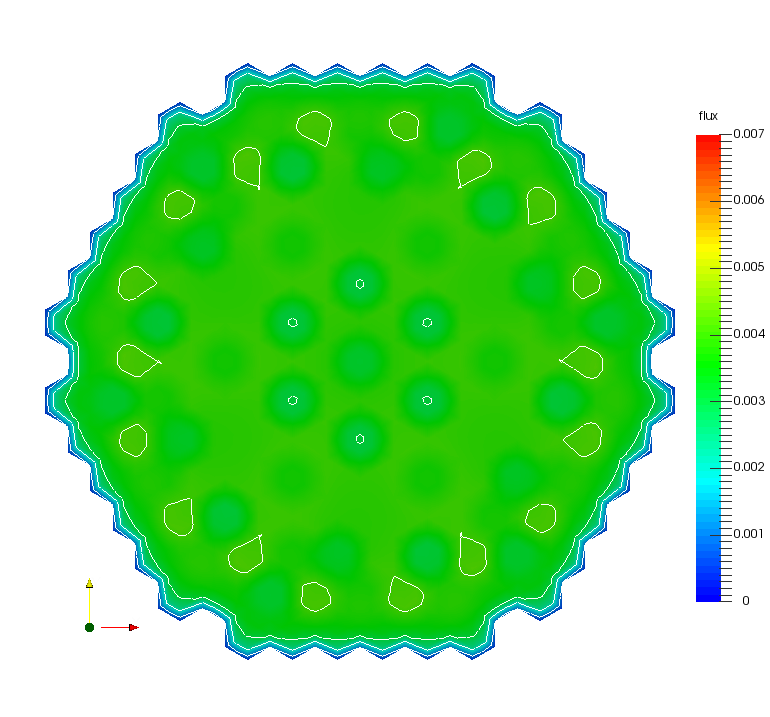
\includegraphics[width=1\linewidth]{18-1.png}} \\
\end{minipage}
\hfill
\begin{minipage}{0.49\linewidth}
\center{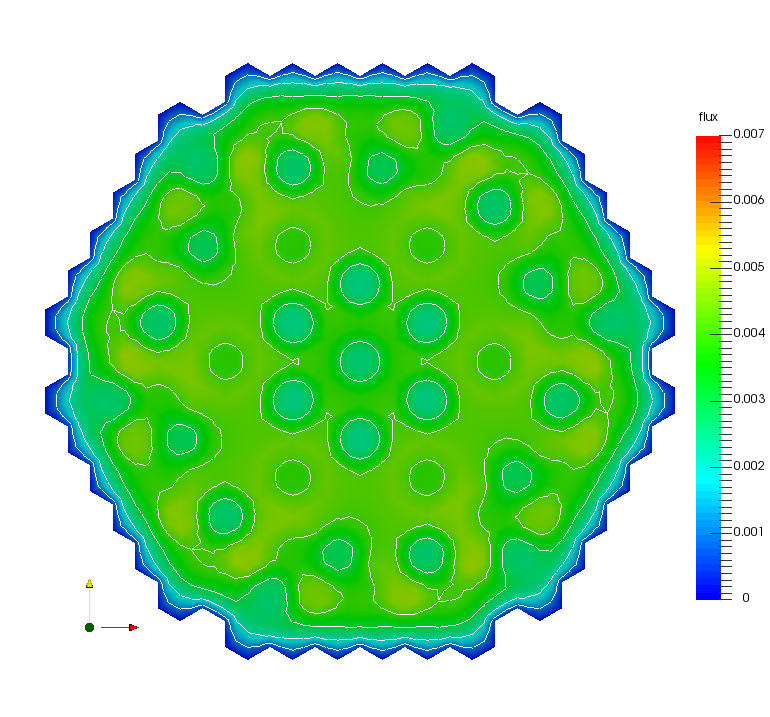
\includegraphics[width=1\linewidth]{18-2.png}} \\
\end{minipage}
\caption{Real part of eigenfunctions $\varphi^{(2)}_1, \ \varphi^{(3)}_1$ (left) and $\varphi^{(4)}_1, \ \varphi^{(5)}_1$ (right).}
\label{fig:18}
  \end{center}
\end{figure}
\begin{figure}[!h]
  \begin{center}
\begin{minipage}{0.49\linewidth}
\center{\includegraphics[width=1\linewidth]{19-1.png}} \\
\end{minipage}
\hfill
\begin{minipage}{0.49\linewidth}
\center{\includegraphics[width=1\linewidth]{19-2.png}} \\
\end{minipage}
\caption{Imaginary part of eigenfunctions $\varphi^{(2)}_1, \ - \varphi^{(3)}_1$ (left) and $\varphi^{(4)}_1, \ - \varphi^{(5)}_1$ (right).}
\label{fig:19}
  \end{center}
\end{figure}

The eigenfunctions for fundamental eigenvalue ($n=1$) of the spectral problem (\ref{18}) are shown in the Fig. \ref{fig:17}.

The real part of the eigenfunctions $\varphi^{(n)}_1, \ n = 2,3,4,5$ is shown in the Figure \ref{fig:18}.
Figure \ref{fig:19} shows the imaginary part of these eigenfunctions.

The first eigenfunctions of the problems (\ref{17}) and (\ref{18}) are close to each other in topology.
The eigenvalues $\lambda_1^{(\alpha)} \leq  \lambda_2^{(\alpha)} \leq ...$
are well separated. In our example, the fundamental eigenvalue is negative and therefore the main harmonic will increase, while all others will attenuate. A regular mode of the reactor is thereby defined. The value $\alpha = \lambda_1^{(\alpha)}$ determines the amplitude of neutron field development and connects directly with reactor period in the regular mode.

\pagebreak
\subsubsection{Solution of Delta  Modes spectral problem} 
The results of solution of this spectral problem for the first five eigenvalues are shown in Table \ref{t-8}. All the eigenvalues are real, and the value $\delta = \delta_1 \approx -1132.82$ is far enough from the value $\alpha  = \alpha_1 \approx 42.26$.
The eigenvalues of the problem (\ref{19}) are of little importance. Therefore only $\varphi^{(1)}_1$ and $\varphi^{(2)}_1$ are given in Figure \ref{fig:20}.

\begin{table}[h]
\caption{The eigenfunctions $\delta_n = 1 / \lambda_n^{(\delta )}, \ n = 1,2,...,5$}
\label{t-8}
\begin{center}
\begin{tabular}{ccccccc}
\rowcolor{col1}
$\kappa$ & $p$ & $\delta_1$ &  $\delta_2$ &  $\delta_3$ &  $\delta_4$ &  $\delta_5$ \\ 
\rowcolor{col3}
   & 1 & -1127.55257 & -1009.80617 & -1009.80398 & -871.60140 & -871.59855 \\
\rowcolor{col2}
6  & 2 & -1132.64216 & -1018.75605 & -1018.75385 & -883.21855 & -883.21571 \\
\rowcolor{col1}
   & 3 & -1132.81177 & -1019.03389 & -1019.03169 & -883.53871 & -883.53587 \\
\rowcolor{col3}
   & 1 & -1131.36452 & -1016.52656 & -1016.52435 & -880.32945 & -880.32661 \\
\rowcolor{col2}
24 & 2 & -1132.80333 & -1019.02010 & -1019.01790 & -883.52291 & -883.52007 \\
\rowcolor{col1}
   & 3 & -1132.82161 & -1019.05019 & -1019.04798 & -883.55788 & -883.55504 \\
\rowcolor{col3}
   & 1 & -1132.44380 & -1018.39826 & -1018.39605 & -882.72667 & -882.72383 \\
\rowcolor{col2}
96 & 2 & -1132.82067 & -1019.04865 & -1019.04644 & -883.55611 & -883.55327 \\
\rowcolor{col1}
   & 3 & -1132.82240 & -1019.05153 & -1019.04932 & -883.55955 & -883.55671 \\
\end{tabular}
\end{center}
\end{table}

\begin{figure}[h]
  \begin{center}
\begin{minipage}{0.49\linewidth}
\center{\includegraphics[width=1\linewidth]{20-1.png}} \\
\end{minipage}
\hfill
\begin{minipage}{0.49\linewidth}
\center{\includegraphics[width=1\linewidth]{20-2.png}} \\
\end{minipage}
\caption{The eigenfunctions $\varphi^{(1)}_1$ (left) and $\varphi^{(2)}_1$ (right).}
\label{fig:20}
  \end{center}
\end{figure}

\pagebreak
\section{Conclusions} 

The spectral problems that may characterize the dynamic neutron field of nuclear reactor are considered. Within the multi-group diffusion approximation, the standard Lambda Modes spectral problem which is related to the definition of k-effective of the reactor core is considered. The Alpha Modes spectral problem is much more informative for considering the dynamic processes. We can relate the dynamics of the reactor at asymptotic stage at long times to fundamental $\alpha$-eigenvalue and  $\alpha$-eigenfunction. A new spectral problem (Delta Modes spectral problem) is formulated, which is connected to self-adjoint part of operator of neutron absorption-generation. Solution of this problem allows making an a priori estimate for neutron field dynamics.

The computational algorithm for approximate solution of the spectral problems is based on a standard finite-element approximation using Lagrange finite elements of  $p=1,2,3$. 
The matrix spectral problem is solved using a scalable and flexible toolkit for the solution of eigenvalue problems SLEPc. Approximate solution accuracy is checked at a sequence of condensing grid using finite elements of varying degrees.

Test calculations are made in two-dimensional approximation for a nuclear reactor VVER-1000 without reflector and HWR problem using two-group diffusion approximation. The first real and complex eigenvalues and eigenfunctions in the Lambda Modes spectral problem are got. A good separability of the eigenvalues in the Alpha Modes spectral problem is identified. The results of the numerical solution of the Delta Modes spectral problem to assess the dynamics of neutron field are given.

\section*{Acknowledgements}

This work was supported by the Russian Foundation for Basic Research (project 16-08-01215).


\bibliography{din, Vas-2016}

\end{document}
